%%%%%%%%%%%%%%%%%%%%%%%%%%%%%%%%%%%%%%%%%%%%%%%%%%%%%%%%%%%%%%%%%%%%%%%%%%%%%%%%%%
%%% Navigation
%%% 
%%%
%%%%%%%%%%%%%%%%%%%%%%%%%%%%%%%%%%%%%%%%%%%%%%%%%%%%%%%%%%%%%%%%%%%%%%%%%%%%%%%%%%
\chapter{Navigation Results} \label{ch:results_navigation}

% The structure of this chapter needs revision.

% What do we have to talk about here?
% Well, I suppose the point of this chapter is to present how well the algorithm worked.
% What is there to present?
% I suppose it should be shown that the algorithm does indeed nav the robot,
% as that is not necessarily assumed in the chapter explaining the navigation.
% Some things you might want to know:
% Qualitatively, how well did it nav the robot?

% Ok, so what can I show?
% I can show pictures of the Nao naving around different environments getting to goals
% I can show what the robot thought his pose was based on the goal.
% I can list the optimal parameters for naving.
% I wish I could have shown laser data, because maybe I could have shown a potential field map.
% Can I show the different parts of what the nav was using? No, because the straight line planner
% and escape strategy was not implemented.
To test the efficacy of the GODZILA algorithm, the Nao humanoid platform was instrumented with
a Hokuyo LIDAR and set in three different arenas to navigate to a goal. The Nao was used as the mobile
base for the experiment while the Hokuyo LIDAR provided range and bearing information about
arena obstacles. The NAOqi API provides functions for tracking a red object using its onboard cameras
to estimate the range and bearing to the object. A red cube was designated as the goal location
that the robot could track. 
A secondary camera was mounted to the ceiling of the room in which the
arena was set up such that the entire arena and progress of the robot could be recorded.
This video was only used to record the results of the experiment and at no time did the robot
have access to this data during the experiment. The relative pose estimates from the Nao about
the goal location were also recorded for analysis.

Details about the Nao and LIDAR can be found in Chapter~\ref{ch:platform} and details about 
the arena setup, data collection, and algorithm parameters can be found in Section~\ref{sec:nav_exp_setup}.
Data collected by the robot about the goal pose is presented in Section~\ref{sec:nav_goal_pose_tracking}
and robot pose data collected by the global camera is presented in Section~\ref{sec:nav_robot_pose_tracking}.

\section{Experimental Setup} \label{sec:nav_exp_setup}
Using the NAOqi API discussed in Chapter~\ref{ch:platform}, the GODZILA algorithm was implemented 
on the Nao in C++. Different arenas were constructed and the robot was set at
some start location and navigated to some radius from the goal location before stopping.
Concurrently, the parameters of the algorithm were tuned such that the robot performed
well in any of the tested arenas. This section discusses the platform hardware
(Section~\ref{subsec:nao_and_lidar}), goal pose estimation (Section~\ref{subsec:goal_pose_est}),
and the tuned GODZILA parameters (Section~\ref{subsec:godzila_params}).
Finally, it overviews the experimental arenas (Section~\ref{subsec:arena}) and the
global camera setup (Section~\ref{subsec:robot_pose_est}) used to record each test.

% Hardware setup.
\subsection{Mobile Platform and LIDAR} \label{subsec:nao_and_lidar}
% the Nao was used, and had a Hokuyo LIDAR stuck to its chest.
% We used Nao's built in walking to walk, which as we'll discuss, sucked (put us at a disadvantage),
% because since we strapped a big mass to it's chest that it didn't know about,
% the thing had a tendency to loose stability and fall over.
% (In fact we couldn't keep going because the fucker kept falling over and breaking it's gears.)

% The LIDAR allowed the Nao to detect obstacles. These LIDAR points fed the algorithm and repelled.
The Nao humanoid platform was used as the mobile base for the experiment.
The NAOqi API provides a bipedal gaiting function that allows the robot to
walk over flat terrain. As the floor of the arena was approximately flat, this gait was
applicable to this experiment and was not modified before use.
To the robot's chest was attached a Hokuyo LIDAR via a 3D printed mount.
The LIDAR had a measurement range between 0.02 and 5.6 meters with an
angular resolution of $0.352^\circ$ and a viewing angle of $\pm 120^\circ$.
Data from this sensor was used by the robot to detect obstacles in the environment.
GODZILA used this data to generate the repulsive force vectors discussed in Chapter~\ref{ch:navigation}.
These repulsive forces allow the robot to avoid colliding with obstacles in the environment.
An in depth discussion of the Nao, LIDAR, and LIDAR mount can be found in 
Chapter~\ref{ch:platform}.
A shortcoming of this approach was that while the LIDAR and mount were physically
compact and well within the load carrying capacity of the Nao platform, the dynamics
generated by moving this additional mass during gaiting were not accounted for by the
in-built walking algorithm as there was no method available to modify the dynamic model.
As a result, the walking gait became marginally stable and at times, unstable.
The marginal stability of the platform can be seen in the results presented in 
Section~\ref{sec:nav_robot_pose_tracking}.
In future work, these additional dynamics will need to be accounted for in order to
increase the robustness of the platform, should it be used again for this or a similar
experiment.


% Goal sensor/Blob detection,
\subsection{Goal Pose Estimation} \label{subsec:goal_pose_est}
The head of the Nao is equipped with two color cameras. The optical axis of the
first camera is nearly collinear with the x-axis of the head, allowing the
robot to see in front of it. The optical axis of the second camera is pitched
down by approximately $40^\circ$, allowing the robot to see objects near it's feet.
The NAOqi API provides functions to track a ``red ball'' using the images from the first camera. 
These functions actuate the head in an effort to keep the ``red ball'' in frame at all times.
The functions also return the position of the ``red ball'' relative to the torso of the robot.
This can be done because the API assumes the diameter of the ball to be $0.06 m$, allowing
the apparent diameter of the ball to estimate the actual diameter.
With this as a tool, a red object was constructed to indicate to the robot the location of the
navigation goal. The object was tracked during navigation and its estimated position was used
by GODZILA to generate the attractive force vector discussed in Chapter~\ref{ch:navigation}.
The red object was built as a cube with sides $0.127 m$ long. The cube was
mounted on a wooden dowel that was nearly as tall as the Nao which was in turn
affixed to a heavy wooden base.
The cube was mounted on the dowel to allow the robot to see it more easily as this
allows the head to minimize the amount of pitching that must be done to keep the cube in view.
The red object was a cube because during testing the ``red ball'' tracking algorithm did not
seem to be affected by the change in geometry and the cube shape was easier to construct.
The cube width was twice as wide as the expected diameter to allow the target to be seen 
by the robot from longer distances. This longer range allowed for the construction of
a larger arena as well as more robust tracking at shorter ranges.
However, the larger object results in an incorrect range estimate of the tracked object.
While this estimation error is rectifiable through appropriate calibration,
during these experiments the corrections were not performed.
This would mean that the algorithm parameters would be different in a calibrated system
and the presented data shows the robot stops roughly twice as far from the goal than as
instructed.
% Also, since we needed to know where the goal was we used the built it blob
% detection on Nao and made up a big red cube for it to detect.
% The stock blob detection not only gives you bearing to a goal but it also assumes that the
% red blob is a certain size (diameter: 0.06 m) and therefore can estimate range to the obstacle.
% While you would think then that we should have used an object that size,
% since we were asking it to track something so far away and cameras suck, we had to use a bigger 
% (0.127 m or 5 inch side length or twice as big)
% object so it could be seen at distance.
% This of course then meant that the range measurement was incorrect, but since we were
% only using the range measurement for the goal attraction and to determine when to stop,
% it wasn't that big of a deal and we could tune around it.

% Now that I think about it, what we should have done was calibrate the distance with this
% object so the tuning for GODZILA and the stopping distance would be ``real'' and not to
% this messed up thing.
% You would definitely definitely definitely have to do this if you were going to do mapping,
% which was the next step.

% The robot was told to stop 0.3 meters radius from the goal.


\subsection{GODZILA Parameters} \label{subsec:godzila_params}
% WHAT ARE THE OPTIMAL PARAMETERS/PARAMETERS USED.
% This table will have to be reduced and most likely added to the appendix in it's
% full form. Also, probably going to have to explain all of these parameters.
% Probably something like, ``we interface with/tune the algorithm through the following parameter''
% and then explain each one in relation to the math or whatever.
The GODZILA algorithm uses a number of tunable parameters to generate vehicle 
navigation commands. Chapter~\ref{subsec:navoptimization} discusses the theoretical
basis for these parameters. Each needs to be experimentally tuned in order
to achieve optimal performance. They can be roughly divided into three categories which
are discussed in this section. The first set is concerned with limits and thresholds
governing navigation performance. The second influences the behavior of the robot while
turning, while the third influences the forward motion of the robot.
While testing the GODZILA implementation, these parameters were tuned according to the
observed behavior during the testing runs. Table~\ref{tab:nav_params1} shows the parameters used
by the algorithm which produced the results presented in this chapter.

\begin{table}
  \centering
  \begin{tabularx}{\textwidth}{|l|X||r|}
    \hline
    \textbf{Category} & \textbf{Parameter Name}  & \textbf{Value}               \\  \hline\hline
    \multirow{7}{*}{Thresholds}     & Goal Stopping Radius         &   0.3  $m$             \\ 
                                    & Minimum Linear Velocity      &  -0.4  $\frac{m}{s}$   \\  
                                    & Maximum Linear Velocity      &   0.4  $\frac{m}{s}$   \\  
                                    & Minimum Angular Velocity     &  -0.2  $\frac{rad}{s}$ \\  
                                    & Minimum Angular Velocity     &   0.2  $\frac{rad}{s}$ \\  
                                    & Clearance Threshold          &   0.3  $m$ \\  
                                    & Obstacle Threshold           &   3.0  $m$ \\  \hline
    \multirow{5}{*}{Turning}        & Goal Attraction              &   100   \\  
                                    & Obstacle Repulsion           &   20    \\  
                                    & Obstacle Attraction          &   0     \\  
                                    & Obstacle-Goal Bearing Ratio  &   1     \\  
                                    & Vehicle Inertia Gain         &   15    \\  \hline
    \multirow{3}{*}{Forward Motion} & Velocity Gain                &   5     \\  
                                    & Obstacle Repulsion           &   5     \\  
                                    & Angular Rate Braking         &   3     \\  \hline
  \end{tabularx} 
  
  \caption{Table of GODZILA parameters and the values used during experimentation.
           Each parameter is divided into categories controlling thresholds, turning, and
           forward motion. While the thresholds have units, the turning and forward motion
           parameters consist of gains and ratios, which have no unit.}
  \label{tab:nav_params1}
\end{table}

\subsubsection{Navigation Thresholds}
Seven parameters limit the navigation performance of the robot to be within certain bounds.
Generally, these parameters exist to ensure the safety of the robot and environment
but their inclusion affects the tuning of the other parameters as they introduce
system non-linearities.

\paragraph{Goal Stopping Radius}
This is the maximum distance the robot can be from the goal point before GODZILA considers
the robot to have reached the goal position. Practically, the robot will never estimate its
range from the goal to be exactly zero, so to prevent the robot from oscillating around the
goal pose, this parameter gives a stopping criteria for navigation.

\paragraph{Minimum Linear Velocity}
This is the minimum linear velocity of the vehicle in $\frac{m}{s}$, which is allowed to be negative.
Minimums were decided we defined this way to allow simple configuration of non-symmetric velocity
limits. 

\paragraph{Maximum Linear Velocity}
This is the maximum linear velocity of the vehicle in $\frac{m}{s}$.

\paragraph{Minimum Angular Velocity}
This is the minimum angular velocity of the vehicle in $\frac{rad}{s}$, which is allowed to be negative.

\paragraph{Minimum Angular Velocity}
This is the maximum angular velocity of the vehicle in $\frac{rad}{s}$.

\paragraph{Clearance Threshold}
This is the minimum acceptable distance between the vehicle and an obstacle.
% Setting this distance does not guarantee that the robot will never violate this threshold.
It is not guaranteed that this threshold will never be violated, rather a very high cost
is associated with traveling this close to obstacles.
This distance is defined as the center of the robot to the center of an obstacle in meters.
This center to center distance is because all objects are modeled as points.

\paragraph{Obstacle Threshold}
% Method for setting the obstacle range at which it is acceptable to treat obstacles
% as attractive rather than repulsive.
Obstacles that are farther from the robot than this distance are treated as attractive
rather than repulsive. This allows the robot to approach obstacles in order to allow
for some degree of environmental exploration and prevents the robot from simply settling in the middle of
the largest expanse. This quantity is measured in meters.

\subsubsection{Turning Parameters}
% Method for tuning the planning parameters for angular velocity. 
Five parameters are used to shape the function used to generate
turning commands for the robot. They affect the attraction and repulsion
to the goal and obstacles as well as dampening oscillations.

\paragraph{Goal Attraction}            
This gain influences the strength of the goal attraction force.
Larger values increase attraction strength. 

\paragraph{Obstacle Repulsion}  
This gain influences the strength of the obstacle repulsion force for 
obstacles closer than the Obstacle Threshold distance.
Larger values increase repulsion strength. 

\paragraph{Obstacle Attraction}        
This gain influences the strength of the obstacle attraction force for 
obstacles farther than the Obstacle Threshold distance.
Larger values increase attraction strength. This predisposes the robot
to point in the direction of far obstacles.

\paragraph{Obstacle-Goal Bearing Ratio}  
This gain tunes the trade off between avoiding obstacles which are in the robot's 
current direction of travel versus avoiding objects which are in the direction of the goal.
This parameters ranges from 1 to 0. 
Values closer to 1 amplify the avoidance of obstacles in the direction of travel.
Values closer to 0 amplify the avoidance of obstacles in the direction of the goal. 

\paragraph{Vehicle Inertia Gain}            
This gain influences the strength of the vehicle's resistance 
to turning. Larger values mean more resistance to turning. This can be seen
as increasing the inertia of the robot and will help dampen high frequency oscillations
associated with intermittent obstacle detection and local minima conditions.
The algorithm is constructed such that forward motion is reduced in the presence of large
angular velocities so high frequency changes in desired heading angle slow the robot down.

\subsubsection{Forward Motion Parameters}
 % Method for tuning the planning parameters for linear velocity.
Three parameters are used to shape the function used to generate forward motion
commands. The term forward motion is used as this function only commands the
robot to move in the direction (or in the opposite direction) of its current heading.
A different function would have to be formulated to take advantage of the planar
holonomy of the Nao humanoid, which would likely have different parameters.

\paragraph{Velocity Gain}              
This gain influences the ``aggressiveness'' of the forward velocity function. 
Larger values effectively increase the slope of this function, meaning the change in
velocity will be greater for a given change in the other input parameters.

\paragraph{Obstacle Repulsion}  
This gain influences the strength of repulsion force generated by the closest obstacle.
Larger values increase repulsion strength.
The strategy here is that the robot should slow down if there are obstacles close to it.
Only the closest obstacle is used to modify forward velocity.

\paragraph{Angular Rate Braking}        
This gain influences the amount by which high turning rates reduce forward velocity.
Larger values reduce forward velocity to a greater extent.
In general, when the robot is trying to turn quickly, it is likely that heading forward in that
direction is no longer desired.

\subsection{Experimental Arena} \label{subsec:arena}
% Brief paragraph intro on what are the three arenas.
% We did three different environments with different environmental features.
% So, as a control basically, one of the environments was just open. Yes there are walls
% so there is a repulsive force but nothing should be obstructing the attraction to the
% goal and if this doesn't work then something is really messed up. Figure \ref{fig:nav_open_setup1}
% shows the setup.
Three arenas were constructed to test the efficacy of the GODZILA algorithm.
In all three, the goal location is observable by the robot at all times as the robot had no other
method to know goal location, nor is there any provision in the GODZILA algorithm for doing
searches or explicit explorations.
The first arena was simply an open area in which the robot could walk towards the goal.
This trivial environment acts as a control in which the robot is always expected to
reach the goal. The second arena contains an obstacle which divides the arena into two
parts such that the only means to reach the goal is through a narrow opening. The objective is
to demonstrate the narrowest opening that can be traversed using this method.
Finally, an arena was constructed which had a large obstacle that would always have a large
local influence on the navigation. The robot must overcome the large repulsive forces
and walk through a hallway to the goal.
In common to the three arenas was a perimeter wall which acted to contain the environment and
prevent the presence of unplanned obstacles from influencing test results. The arena perimeter
was approximately $11.75 m$ long by $5.5 m$ wide. As an aside, none of the perimeter walls are
depicted in any of the figures seen in this chapter. This is simply an aesthetic choice and are
present in each experiment.
% The outer perimeter of the arena way yay big. The LIDAR range was 5 meters, so having the
% perimeter, which was all straight flat walls, meant that the robot could always see them.
% This let things be consistent when testing, thought not strictly necessary for the algorithm to
% work as the robot doesn't need to localize in order to navigate.
% You don't see these walls in the figures, for aesthetic reasons.

\subsubsection{Arena Construction}
% Everything was boxy since that was the easiest shape to put together that had the
% same 2D projection throughout. We could only test things at laser height and obstacles
% like chairs which can have things jutting out above and below the laser are obviously going
% to mess things up because the robot can't see them, so there really wasn't a point to testing
% that.
The arenas were constructed using large cuboidal objects and flat walls. Aside from the ease of
construction, this is motivated by the choice of sensor used on the robot for obstacle avoidance.
The cuboids and walls have the same cross section when viewed from above. As the LIDAR used
only detects objects in a plane, obstacles which have overhangs or voids at different levels
are effectively invisible to the robot and pose a collision risk. This is not a shortcoming of
the algorithm but rather the sensor, therefore, using obstacles that avoid this risk is appropriate.

% Maybe we could have had more thin objects but then we're talking about the laser resolution
% constraint. This would probably be a good one to try next time since it falls in the range of
% detectability though it's sort of now in the obstacle avoidance part of things
% which should be it's own algorithm in the stack of things to do all of navigation.

% Description of Open Arena.
\subsubsection{Open Arena}
% So, as a control basically, one of the environments was just open. Yes there are walls
% so there is a repulsive force but nothing should be obstructing the attraction to the
% goal and if this doesn't work then something is really messed up.
The open arena contained no obstacles and only the arena perimeter walls and the goal
object were present to affect the navigable path.
Figure~\ref{fig:nav_open_setup1} shows a picture of the arena as seen by the overhead camera.

\begin{figure}
  \includegraphics[width=\textwidth]{nav/open/no_path/frame1.png}
  \caption{This figure shows the open arena. The Nao can bee seen on the left at the starting location
           while the goal cube can be seen to the right.
           }
  \label{fig:nav_open_setup1}
\end{figure}

% Description of Narrow Arena.
\subsubsection{Narrow Opening Arena}
% Next we tried one that had a narrow opening between the robot and the goal.
% The opening is about 73 cm wide.
% This opening is about 2.6 times the width of the body of the robot (27.5 cm wide).
This arena contains an obstacle that divides the area into two equal
parts, with the robot and goal being in opposing partitions. The only path between
the two rooms is a narrow opening that is $73 cm$ wide. This width is approximately
2.6 times the shoulder-to-shoulder width of the robot. 
Figure~\ref{fig:nav_narrow_setup1} shows the arena with the narrow opening.
The objective was to demonstrate the narrowest opening that the robot could travel through with this method.
It was found than openings narrower than this caused the robot to approach other obstacles too 
closely when the parameters were tuned to allow the robot to traverse this aperture.
At times, with the parameters tuned to allow for tighter openings, the robot would
collide with corners it might otherwise have avoided.
To allow for the navigation of narrower openings that are still physically traversable,
one strategy is to have a global path planner that could place intermediate goals
to ``pull'' the robot through. As GODZILA is designed to be a lightweight local algorithm,
such provisions are inappropriate for addition to the approach as they tend to require maps.
The different algorithm classes and approaches are reviewed in Chapter~\ref{ch:navigation}.
% It was more or less the
% limit of this approach because if we allow the robot to get closer to obstacles it tends
% to cut too close to corners and other things and mess up.

% To solve this, you'd need something that plans paths though these narrow but traversable
% areas and have intermediate goals along this path for GODZILA to use.
% These would then ``pull'' the robot through the narrow opening.
% This is how the straight line planner works when the goal is in sight.
% That's not the case in the setup so the straight line planner cannot be invoked.
% Also, that's again not really the focus of this algorithm and as mentioned in
% Chapter \ref{ch:navigation}, the responsibility of some global planner.
% Figure \ref{fig:nav_narrow_setup1} shows the setup.

\begin{figure}
  \includegraphics[width=\textwidth]{nav/narrow/no_path/frame1.png}
  \caption{This figure shows the arena with the narrow opening between partitions.
           The opening is approximately 2.6 times the width of the robot and represents
           the practical limit to the traversable apertures using this approach.
           The Nao can bee seen on the left at the starting location
           while the goal cube can be seen to the right.}
  \label{fig:nav_narrow_setup1}
\end{figure}

% Description of Square Arena.
\subsubsection{Large Obstacle Arena}
% Finally, we invoked a more complicated geometry where the robot had to go around
% a large obstacle. In this case, the robot is always relatively close to obstacles and the
% being pushed. Despite the constant repulsion, the goal is attractive enough to
% pull the robot to the goal. Figure \ref{fig:nav_square_setup1} shows the setup.
This arena contained the largest single obstacle possible while still allowing the arena
to be traversable. It consists of a corridor constructed to be the minimum width
a hallway can be with this approach. The corridor also has two $90^\circ$ turns.
The objective was to have the robot navigate in an area where the repulsion of obstacles
was a strong influence during the entire path. It shows that while the robot is constantly being
repelled, it can use the goal and far obstacle attraction to find a path.
Figure~\ref{fig:nav_square_setup1} shows the arena.

\begin{figure}
  \includegraphics[width=\textwidth]{nav/square/no_path/frame1.png}
  \caption{This figure shows the arena containing a large obstacle. The result is a hallway
           that is the narrowest constructible and still have this approach be viable. This results
           in the robot being under strong repulsion for the length of the path.
           The Nao can bee seen on the left at the starting location
           while the goal cube can be seen to the right.}
  \label{fig:nav_square_setup1}
\end{figure}

\FloatBarrier
% Discuss global camera and path estimation analysis.
\subsection{Robot Pose Estimation} \label{subsec:robot_pose_est}
% Hey! Also! The whole thing was recorded with a global camera (A GoPro).
% Having a fixed camera like this is good because it makes tracking the robot
% to measure it's performance trivial.
% We used some image processing to track the Nao's orangeness, clustered to
% find the Nao-like things that were being tracked in the image,
% and then fit a 5th order polynomial curve to it to estimate the path of the
% robot.
In order to track the robot's path for later analysis, a GoPro camera
was mounted on the ceiling above the arena that could record the starting and goal
location in the same frame. This meant that the camera could remain fixed throughout the
experiment, simplifying later analysis.
As presented in Section~\ref{sec:nav_robot_pose_tracking}, this data was processed
using the OpenCV library in Python to track the Nao through the video and display
the path of the robot for each experiment.
 


\section{Goal Pose Tracking} \label{sec:nav_goal_pose_tracking}
% I REALLY have no idea what these are suppose to do for you, but here they are.
% This is what the Nao ``saw'' of the goal while it was walking.
During navigation, the robot used its camera to track the goal location relative to
the robot as discussed in Section~\ref{subsec:goal_pose_est}. 
% Figures \ref{fig:nav_open_rb1}, \ref{fig:nav_narrow_rb1}, and \ref{fig:nav_square_rb1} show
% the range and bearing of the goal as tracked by the Nao during the three experiments.
Figure~\ref{fig:nav_open_rb1} shows the perceived relative goal range and bearing during the open arena
experiment while Figures~\ref{fig:nav_narrow_rb1} and~\ref{fig:nav_square_rb1} show the results from the
narrow opening and large obstacle experiments.
% The ranges are asymptotically decreasing like you would think they would do if the robot
% was getting closer. This doesn't technically have to happen if the robot can ``slide''
% along a straight wall for awhile where it could get a little longer for a bit or in a situation
% where the range stays constant for awhile like a radial wall?
All three datasets show the goal range data following an approximate asymptotic decrease over time.
This is expected as in each of the arenas the robot gets closer to the goal in each step.
While these datasets demonstrate this occurrence, in general there are some arenas where the range
could be constant for a time or even increase slightly. In the presence of a long obstacle that was
radially constant from the goal, the range would constant. Alternatively, if there was a short wall
that was in the path of the goal, the range could increase as the robot avoids it.

% One thing to note is though that the range could never really increase significantly.
% Like if the robot had to go around something that made it walk away, that would never happen.
% The robot would be stuck in this local minima like we talked about in one of the sections of Chapter
% \ref{ch:navigation}.
% We'd have to use some sort of escape strategy.

% The angle doesn't really tell you much since it's the relative bearing which is important to the robot
% but hard for use to interpret since we don't know the global orientation of the robot.
The goal bearing angle in the open arena converges to a small value during the majority of the experiment
while in the narrow opening and large obstacle experiments, the bearing can be seen as oscillating
around some slowly decreasing function. In all of the experiments, the robot is initially oriented facing the goal
to ensure strong goal tracking. In the open arena, this means the robot is already nearly optimally oriented
to approach the goal, and only small corrections to heading are necessary to reach the goal.
In the narrow opening and large obstacle arenas, the robot must first turn away from the goal to
avoid obstacles before the robot can start to face the goal again. Figures~\ref{fig:nav_narrow_frames1}
and~\ref{fig:nav_square_frames1} give additional insight into this process.
The oscillations are likely due to a combination of corrections to the navigation process
and to large head movement due to gaiting oscillations. Section~\ref{sec:nav_robot_pose_tracking} gives
more insights to these gaiting oscillations, due to the added LIDAR mass discussed in 
Section~\ref{subsec:nao_and_lidar}.

% The best we can say is that in one of them (the open area one which makes sense since it had plenty of
% time to get a lock on things and ride the pipe in) it's like always decreasing so he's homing in on things
% and in the others it's oscillating back and forth so it's marginally stable or
% looks like it's some other type of stability like lyapunov or some other thing, which you could
% say means he's got a good track on things.

% I mentioned before that the robot was commanded to stop at 0.3 meters but actually stops closer
% to 0.8 meters because of the perception mismatch.
% In the figures \ref{fig:nav_open_rb1}, \ref{fig:nav_narrow_rb1}, and \ref{fig:nav_square_rb1},
% you can see that the robot thinks it's stopping at the appropriate distance
% of 0.3 meters.
In Figures~\ref{fig:nav_open_rb1}, \ref{fig:nav_narrow_rb1}, and~\ref{fig:nav_square_rb1},
it is also shown that the final perceived goal range is close to the $0.3 m$ prescribed by the Goal Stopping
Radius from Table~\ref{tab:nav_params1}. Section~\ref{sec:nav_robot_pose_tracking} shows that the robot
stopped at a radius closer to $0.8 m$, a mismatch generated by the lack of calibration mentioned in
Section~\ref{subsec:goal_pose_est}.

% Actually, since the goal is not moving, then we probably could do better with the orientation data
% to tell us the orientation of the robot. It's not worth it for this thesis but we could run it through
% some filters and get something to work. We'd either have to EKF it with the initial pose or PF it.
% Not really part of the thesis, but then it makes sense to have analyzed the data because then we could
% use it as the ground truth for a localization algorithm (like Agraj did).
Additionally, a future application of this data is to localize the robot during the experiment. 
This localization data could be used to inform other path planning algorithms or trap detection schemes to improve navigation in more complex
environments.

\begin{figure}
  \centering
  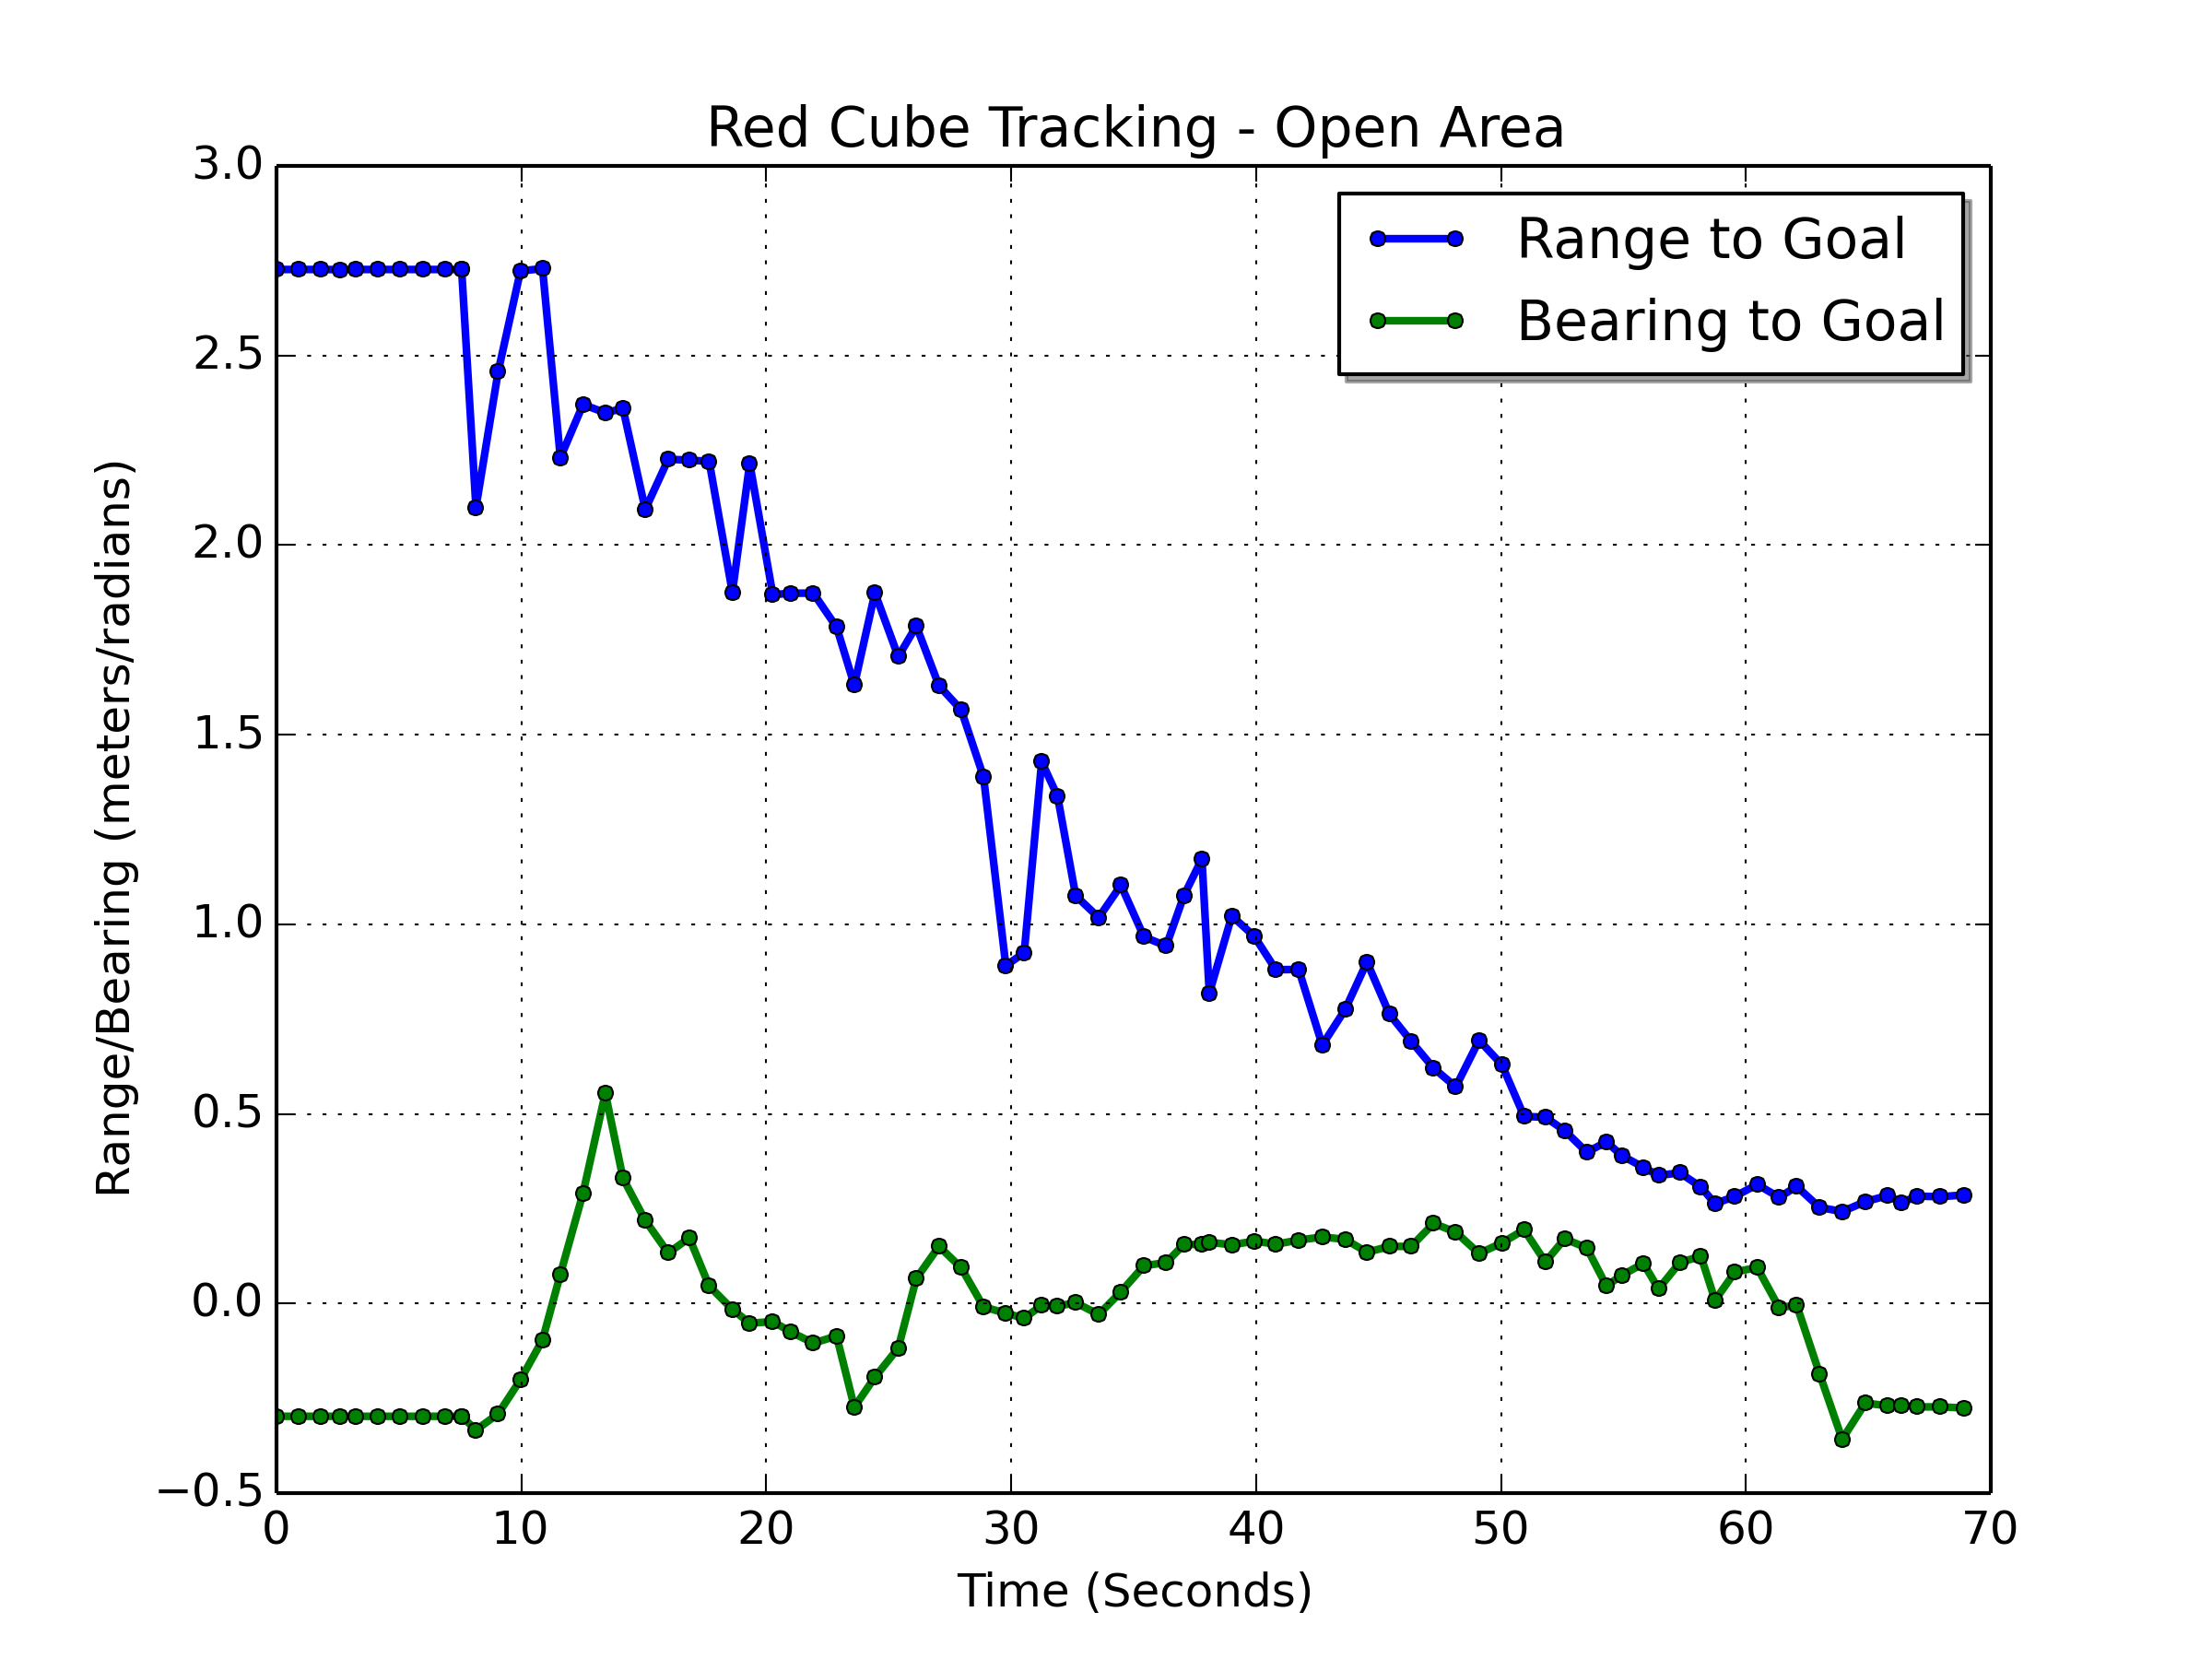
\includegraphics[height=0.35\textheight]{nav/open/tracking/open_rb1.png}
  \caption{This figure plots the perceived range and bearing to the goal
           relative to the robot during the open arena experiment. The range
           to the goal decreases until the Goal Stopping Radius is reached.}
  \label{fig:nav_open_rb1}
\end{figure}

\begin{figure}
  \centering
  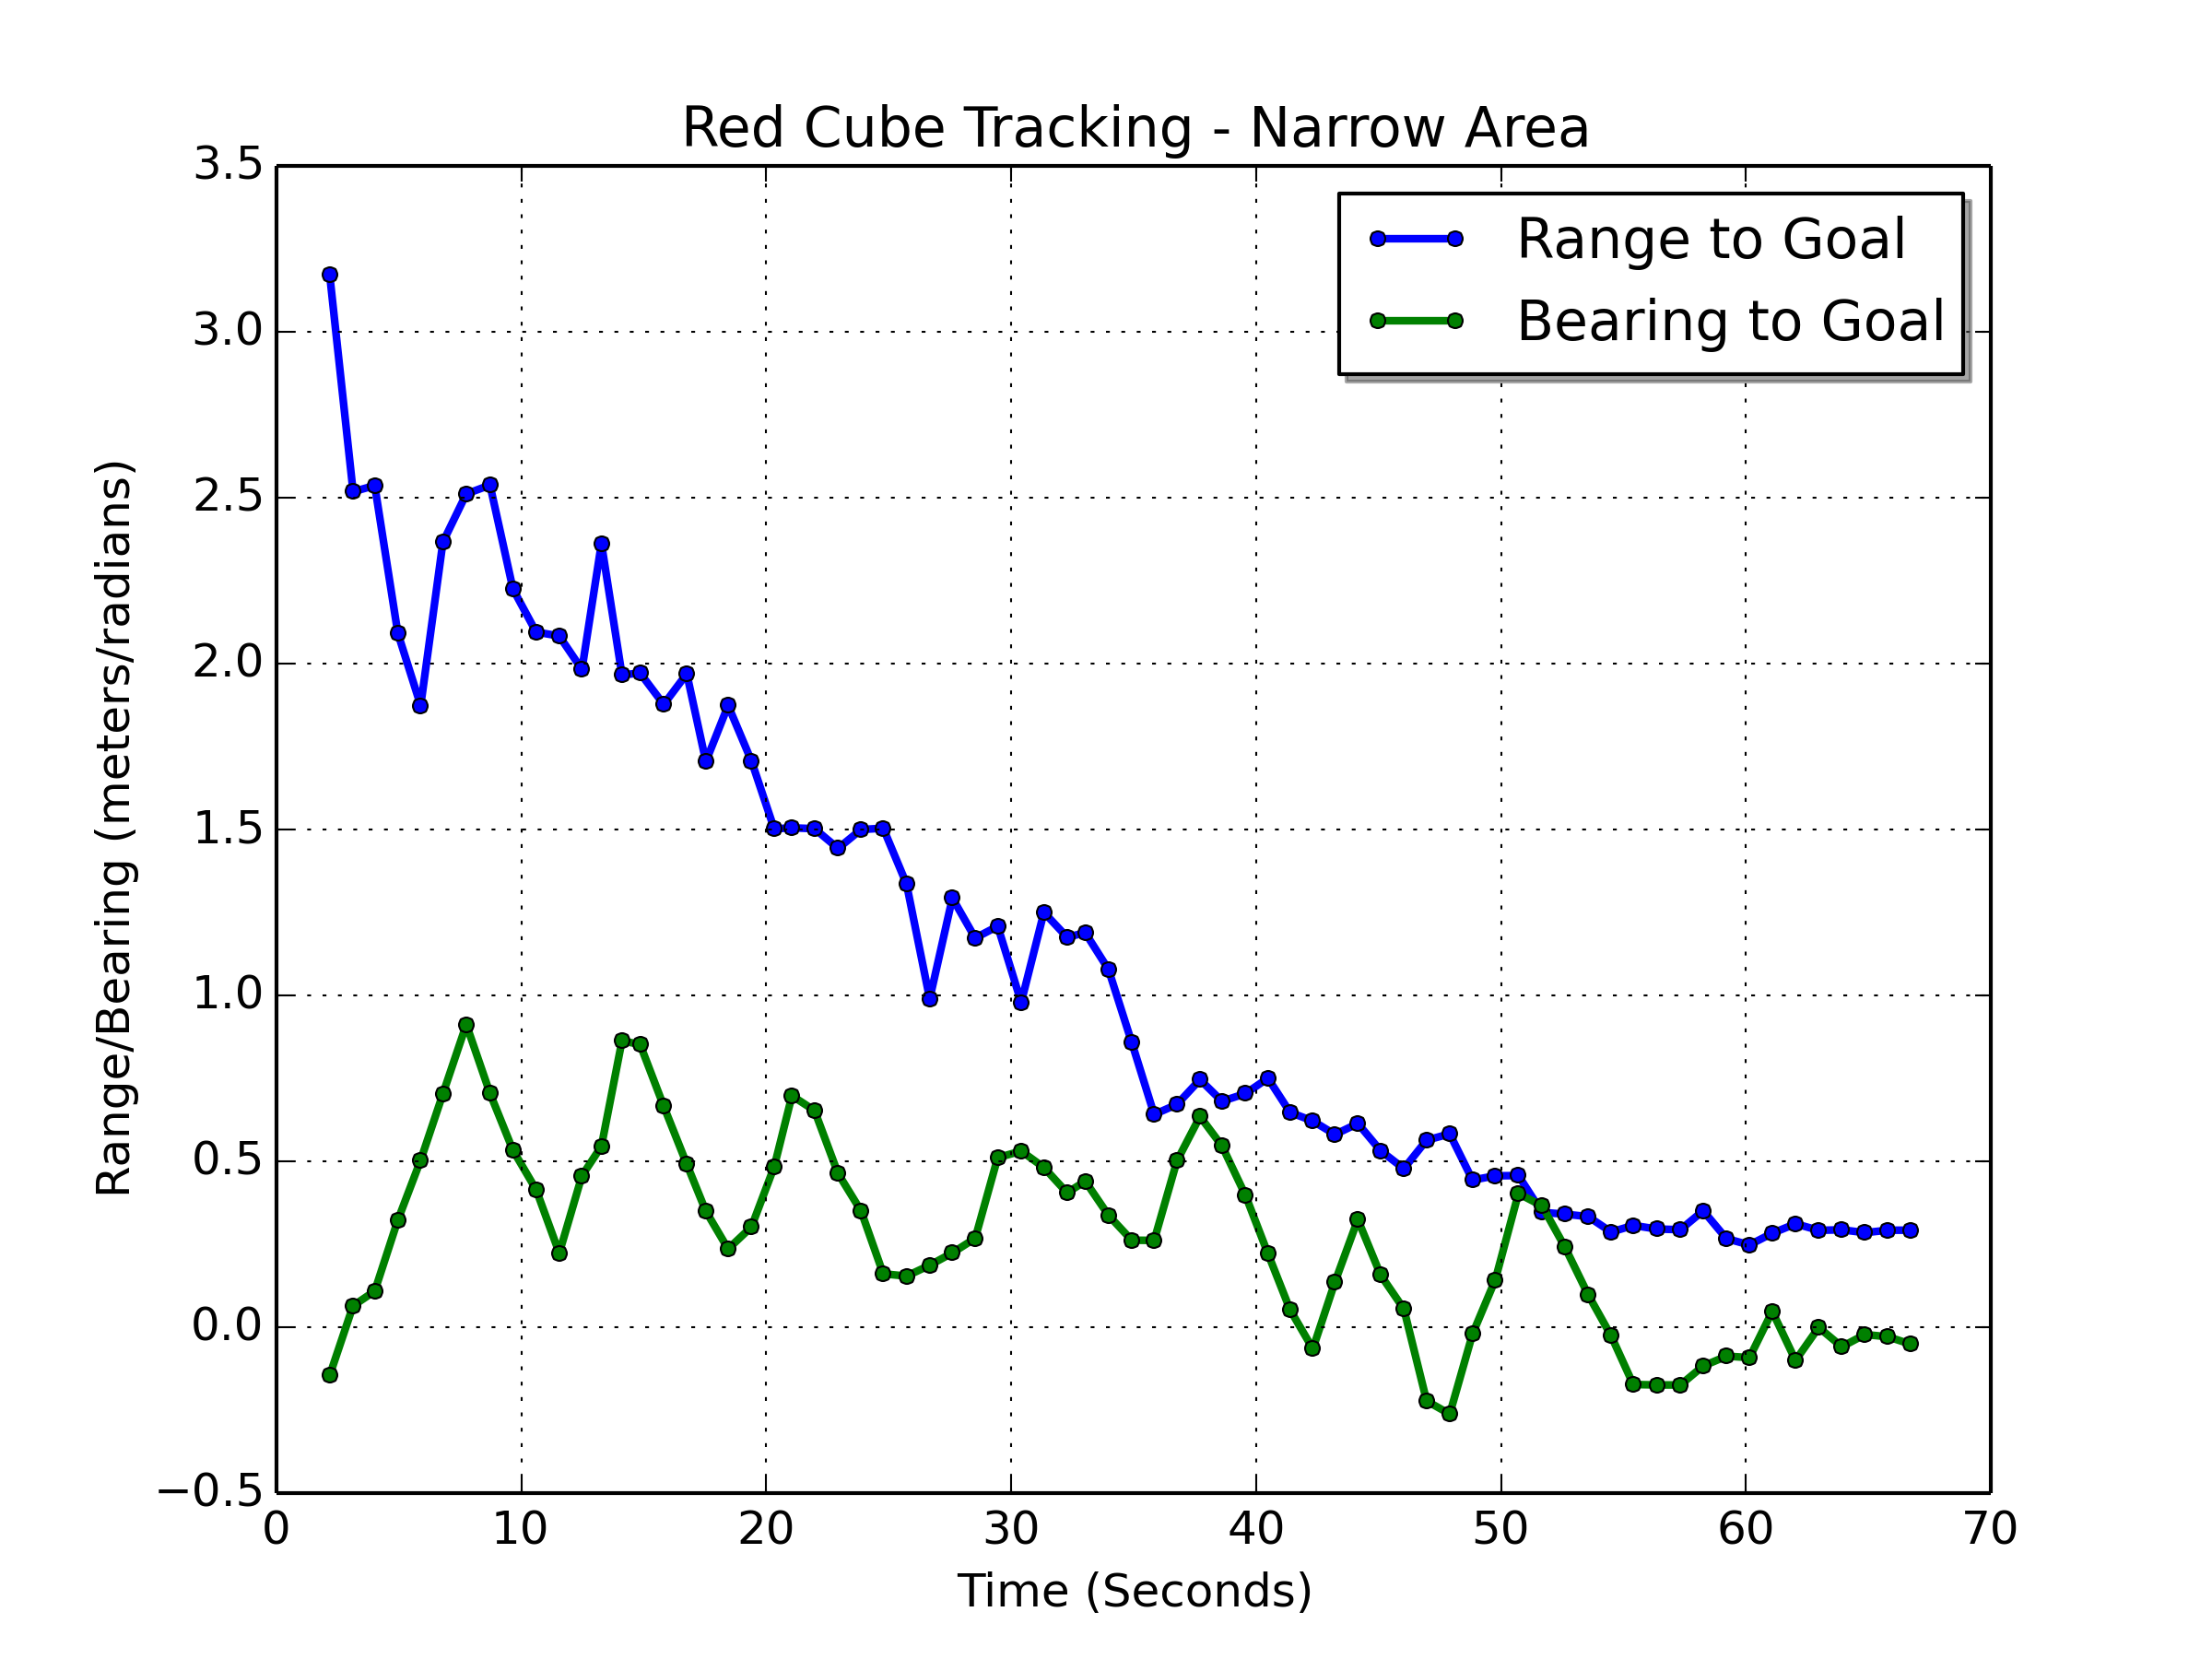
\includegraphics[height=0.35\textheight]{nav/narrow/tracking/narrow_rb1.png}
  \caption{This figure plots the perceived range and bearing to the goal
           relative to the robot during the narrow opening arena experiment. The range
           to the goal decreases until the Goal Stopping Radius is reached.}
  \label{fig:nav_narrow_rb1}
\end{figure}

\begin{figure}
  \centering
  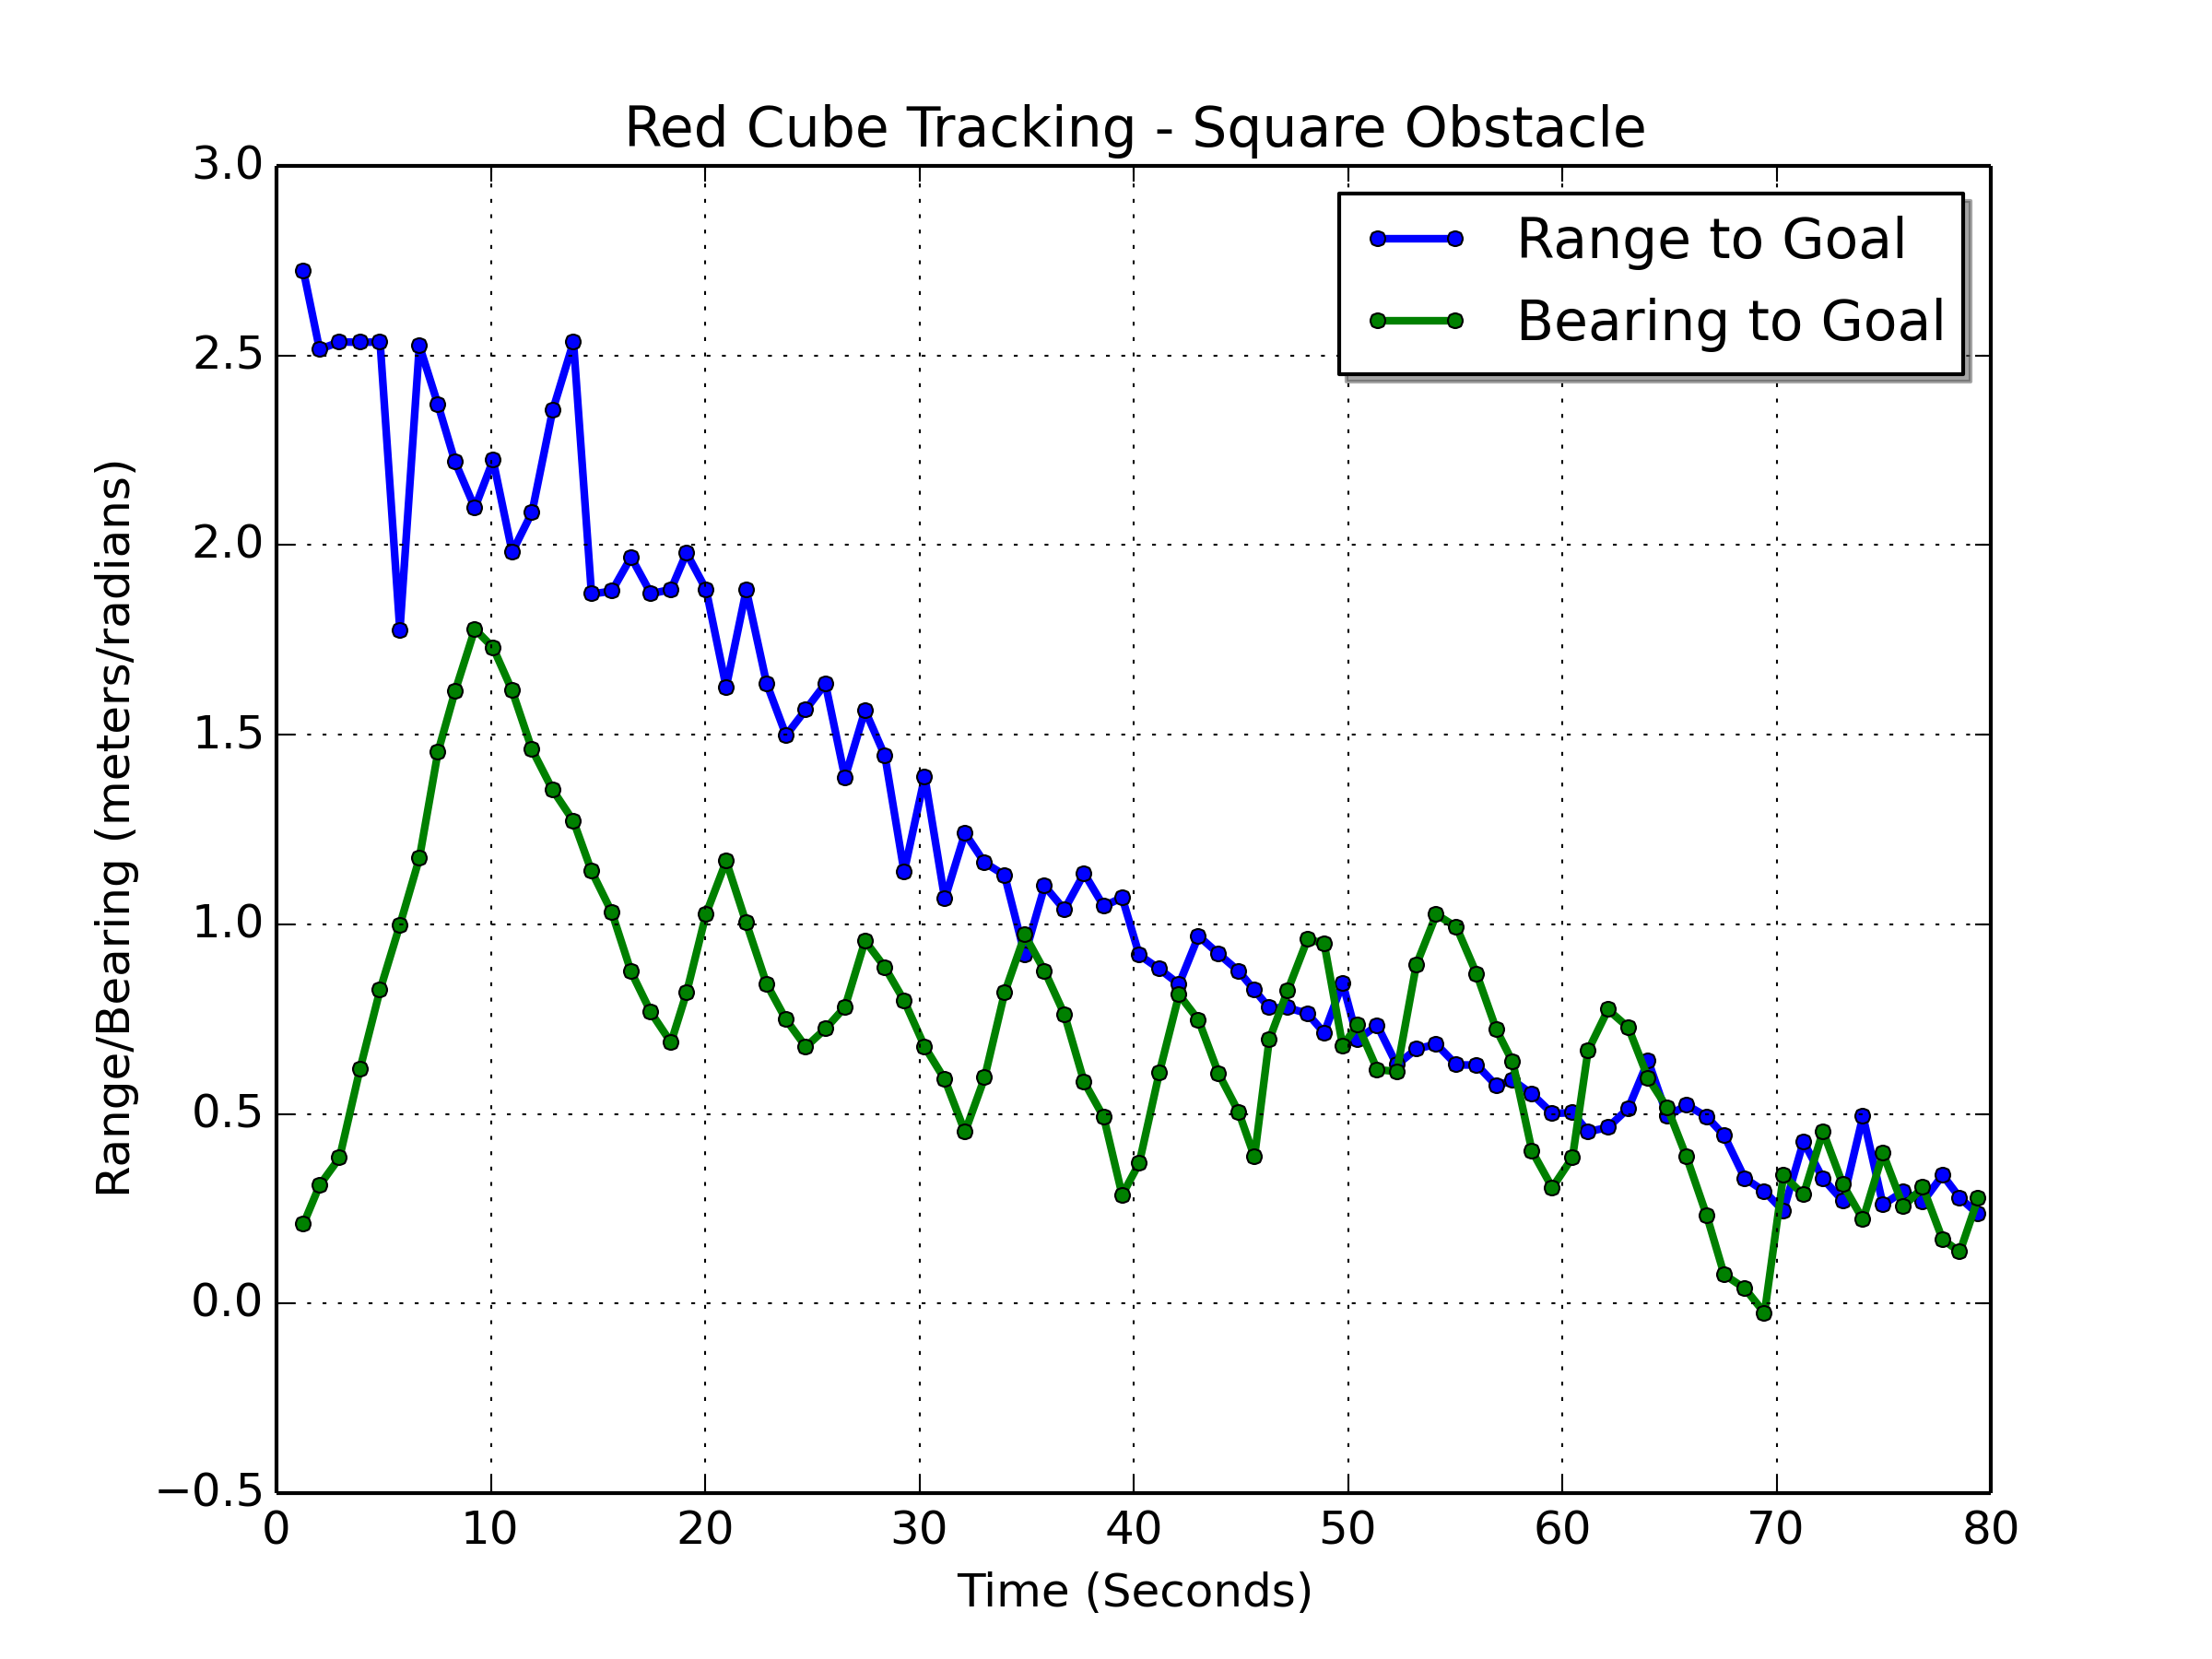
\includegraphics[height=0.35\textheight]{nav/square/tracking/square_rb1.png}
  \caption{This figure plots the perceived range and bearing to the goal
           relative to the robot during the large obstacle arena experiment. The range
           to the goal decreases until the Goal Stopping Radius is reached.}
  \label{fig:nav_square_rb1}
\end{figure}


\FloatBarrier
\section{Robot Pose Tracking} \label{sec:nav_robot_pose_tracking}
In order to record the pose of the robot during the experiments, a GoPro camera
was mounted above the arena. This global camera could see the entire arena during
the experiment, simplifying path analysis. The resultant videos show the robot
traversing from the start location to the goal location while avoiding obstacles.
The video was then analyzed to extract the approximate location of the robot
in each frame and a path was produced from these samples.

\subsection{Observed Path}

% Basically, these pictures are here just to show you that the robot
% made it through the environment. It's not strictly necessary but you wouldn't
% believe me otherwise and they're pretty to look at.
% For convenience, I overlaid the best fit path from the image analysis just
% so you could see ``where'' Nao was going and to give continuity to what you
% are looking at.
As recorded by the global camera during the experiments, Figures~\ref{fig:nav_open_frames1},
\ref{fig:nav_narrow_frames1}, and~\ref{fig:nav_square_frames1} show the robot
as in traverses the arenas. The best fit path, explained in Section~\ref{subsec:tracking_analysis},
is overlaid over each frame to better demonstrate the progression of the robot 
through the arena. In each of the experiments, the robot can be seen navigating
from its starting position, to some position near the goal cube, while avoiding
collision with obstacles. The robot does not approach the obstacles too closely,
nor does it wander in the open areas. An issue that can be seen in each of the
experiments, is the camera parallax between the head and feet of the robot as well
as the goal cube and stand. This effect exaggerates the farther an object is from
the center of the frame. As the best fit path is a result of tracking the orange part
of the Nao during the experiment, the path is distorted. This is especially
apparent in Figure~\ref{fig:nav_square_frames1}, where the path towards the bottom
of the image seems to be farther from the obstacles than one might expect.

\begin{figure}
  \centerline{
    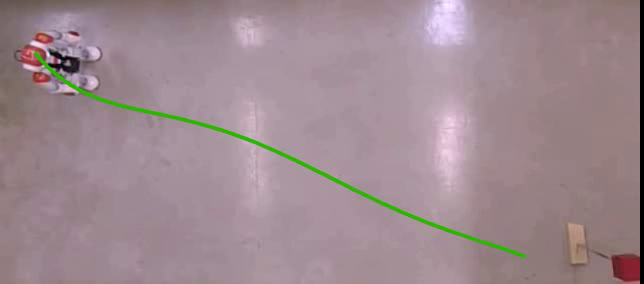
\includegraphics[width=0.5\textwidth]{nav/open/path/open_path1.png}
    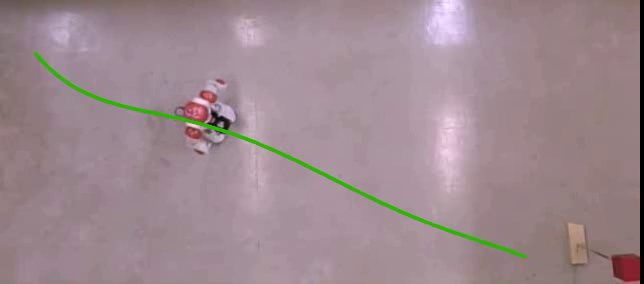
\includegraphics[width=0.5\textwidth]{nav/open/path/open_path2.png}
  }
  \vspace*{0.05in}
  \centerline{
    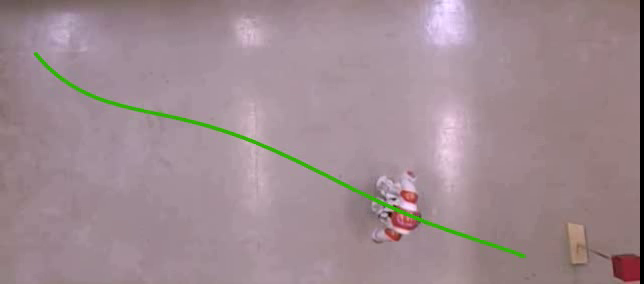
\includegraphics[width=0.5\textwidth]{nav/open/path/open_path3.png}
    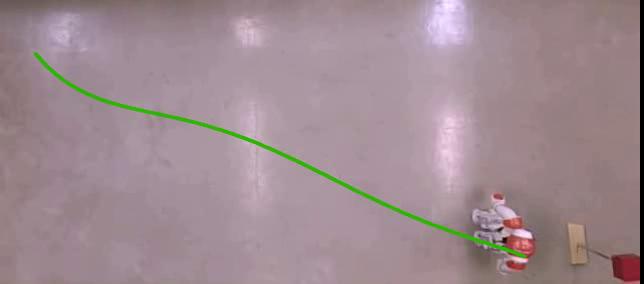
\includegraphics[width=0.5\textwidth]{nav/open/path/open_path4.png}
  }
  \caption{These images show the robot as it progresses through the open arena. 
           The path of the robot is overlaid onto each of the images.
           The robot moves along a straight path to the goal.}
  \label{fig:nav_open_frames1}
  \vspace*{-0.07in}
\end{figure}

\begin{figure}
  \centerline{
    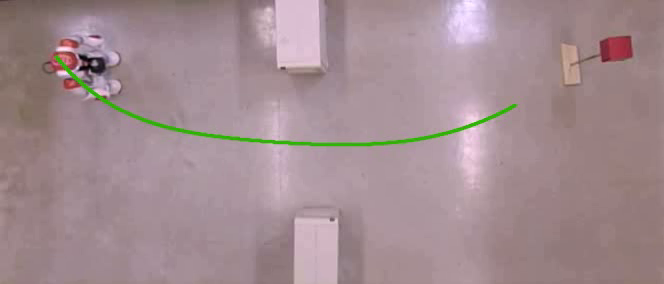
\includegraphics[width=0.5\textwidth]{nav/narrow/path/narrow_path1.png}
    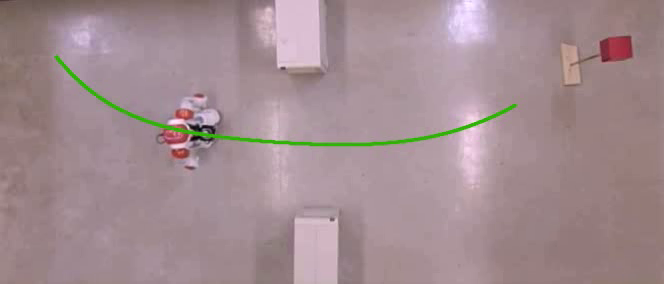
\includegraphics[width=0.5\textwidth]{nav/narrow/path/narrow_path2.png}
  }
  \vspace*{0.05in}
  \centerline{
    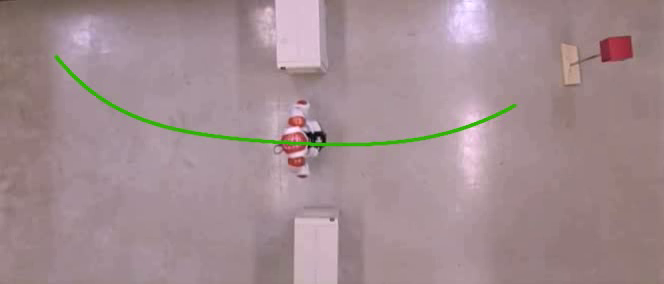
\includegraphics[width=0.5\textwidth]{nav/narrow/path/narrow_path3.png}
    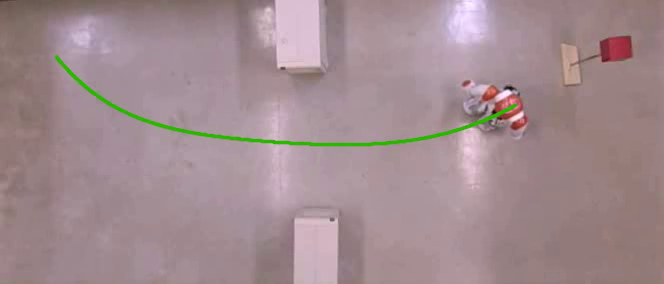
\includegraphics[width=0.5\textwidth]{nav/narrow/path/narrow_path4.png}
  }
    \caption{These images show the robot as it progresses through the narrow opening arena. 
             The path of the robot is overlaid onto each of the images.
             The robot moves towards the middle of the narrow opening and then towards the goal.}
    \label{fig:nav_narrow_frames1}
        \vspace*{-0.07in}
\end{figure}

\begin{figure}
  \centerline{
    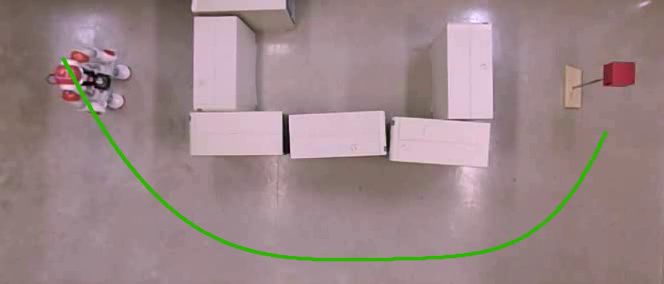
\includegraphics[width=0.5\textwidth]{nav/square/path/square_path1.png}
    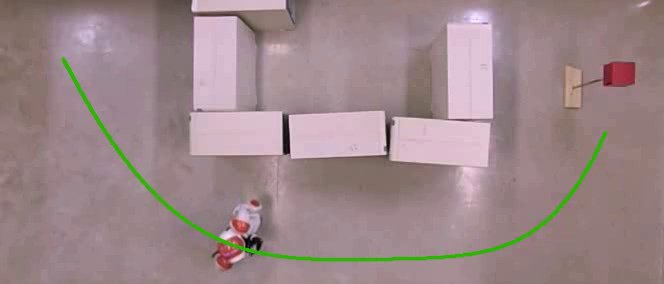
\includegraphics[width=0.5\textwidth]{nav/square/path/square_path2.png}
  }
  \vspace*{0.05in}
  \centerline{
    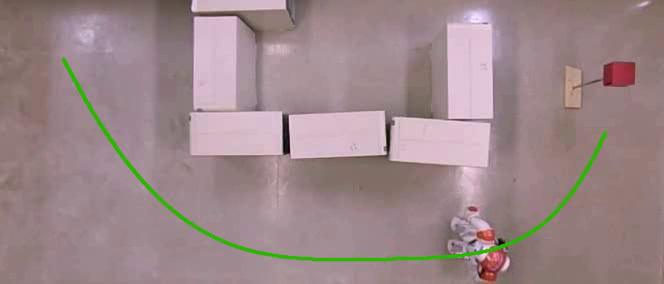
\includegraphics[width=0.5\textwidth]{nav/square/path/square_path3.png}
    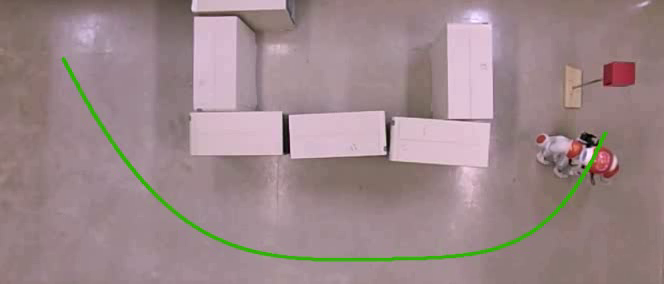
\includegraphics[width=0.5\textwidth]{nav/square/path/square_path4.png}
  }
    \caption{These images show the robot as it progresses through the large obstacle arena. 
             The path of the robot is overlaid onto each of the images.
             The robot moves down from its starting location, along the corridor, and to the goal.
             Camera parallax distorts the path and makes it seem that the robot walks farther away
             from the obstacles during the middle of the run. The upper-right and lower-left images
             show that this is not the case.}
    \label{fig:nav_square_frames1}
        \vspace*{-0.07in}
\end{figure}

\FloatBarrier
\subsection{Tracking Analysis} \label{subsec:tracking_analysis}
% These are what comes out of the image processing.
% I guess I should tell you that I used OpenCV to do blob tracking, some dilations, near cluster
% joining (like the head and shoulders show up as 3 orange blobs so they are joined to estimate the
% center of the robot), then density based clustering to see which ones belong to which (the red cube is
% orange enough to register as something to track so instead of trying to tune the fuck out of the colors
% or use some other technique like template-matching or something I don't know about yet since I'm just 
% starting to use OpenCV), I opted to do clustering and then I manually select which cluster of points are
% the Nao's. Then I used a 5th order polynomial to fit the path.
Using the global camera data from each of the experiments, the robot was tracked through
each video to produce an approximation to the navigated path. The OpenCV library was used to 
process the images in Python. Briefly, the procedure used to produce the path from each video was:

\begin{enumerate}
  \item Extract orange pixels from frame into a new image.
  \item Filter that image using a closing kernel to reduce noise.
  \item Find centroids of remaining pixel ``blobs''.
  \item Eliminate blobs with small areas and join nearby blobs.
  \item Process every video frame to produce array of centroids.
  \item Group centroids using a density-based clustering algorithm.
  \item Manually select the group corresponding to the robot path.
  \item Fit a polynomial to the centroid clusters as the robot path estimate using least-squares.
\end{enumerate}

A fifth-order polynomial was used to approximate the path of the robot because it was the lowest order polynomial fitting that produced a good result.
The results from this procedure can be seen in Figures~\ref{fig:nav_open_plot1},
\ref{fig:nav_narrow_plot1}, and~\ref{fig:nav_square_plot1} for the open arena, narrow opening
arena, and large obstacle arena, respectively. The centroid samples and best-fit path are
overlaid onto one another to show how the path approximates the path of the robot from the
samples. In these plots, the samples clearly illustrate the oscillations in the walking gait.
While every bipedal gait will produce some oscillations in the center-of-mass motion,
the gait instabilities are amplified by the addition of the LIDAR mass as discussed in 
Section~\ref{subsec:nao_and_lidar}. This effect is especially evident in Figure~\ref{fig:nav_narrow_plot1}
towards the middle of the plot. This corresponds to the area near the left side of the narrow
opening. While it is not known why the magnitude of the oscillations at this point are so large,
it is possible that they are not due to the nearby obstacle but due to an irregularity in the
arena floor in this region. This is theorized because the large obstacle arena contained apertures
which were the same width as the narrow opening. Despite this, Figure~\ref{fig:nav_square_plot1} 
does not show any oscillations approaching the magnitude of those seen in Figure~\ref{fig:nav_narrow_plot1}.
% Again, I'm not really sure why you need to see this other than to say here's an analysis of 
% what the robot did that's a little more than just straight pictures.
% You can really see the periodicity in the gait on these graphs.

% You should notice here that while the robot was told to stop at 0.3 m, it actually
% stops closer to 0.8 m from the goal.
% This is because of the mismatch between how big the robot thinks the red object is
% and the fact that it's about twice as big.
Lastly, as mentioned in Section~\ref{subsec:goal_pose_est}, despite the Goal Stopping
Radius from Table~\ref{tab:nav_params1} being $0.3 m$, the robot stops approximately
$0.8 m$ from the goal. This is close to double the parameter value, which is what was predicted
as the cube was about twice as big as the ``red ball'' tracker expected it to be.
The apparent size of the cube when approached from one of the corners, seen with greatest
effect during the narrow opening experiment, would have also contributed to the robot
stopping farther from the goal than intended.

\begin{figure}
  \centering
  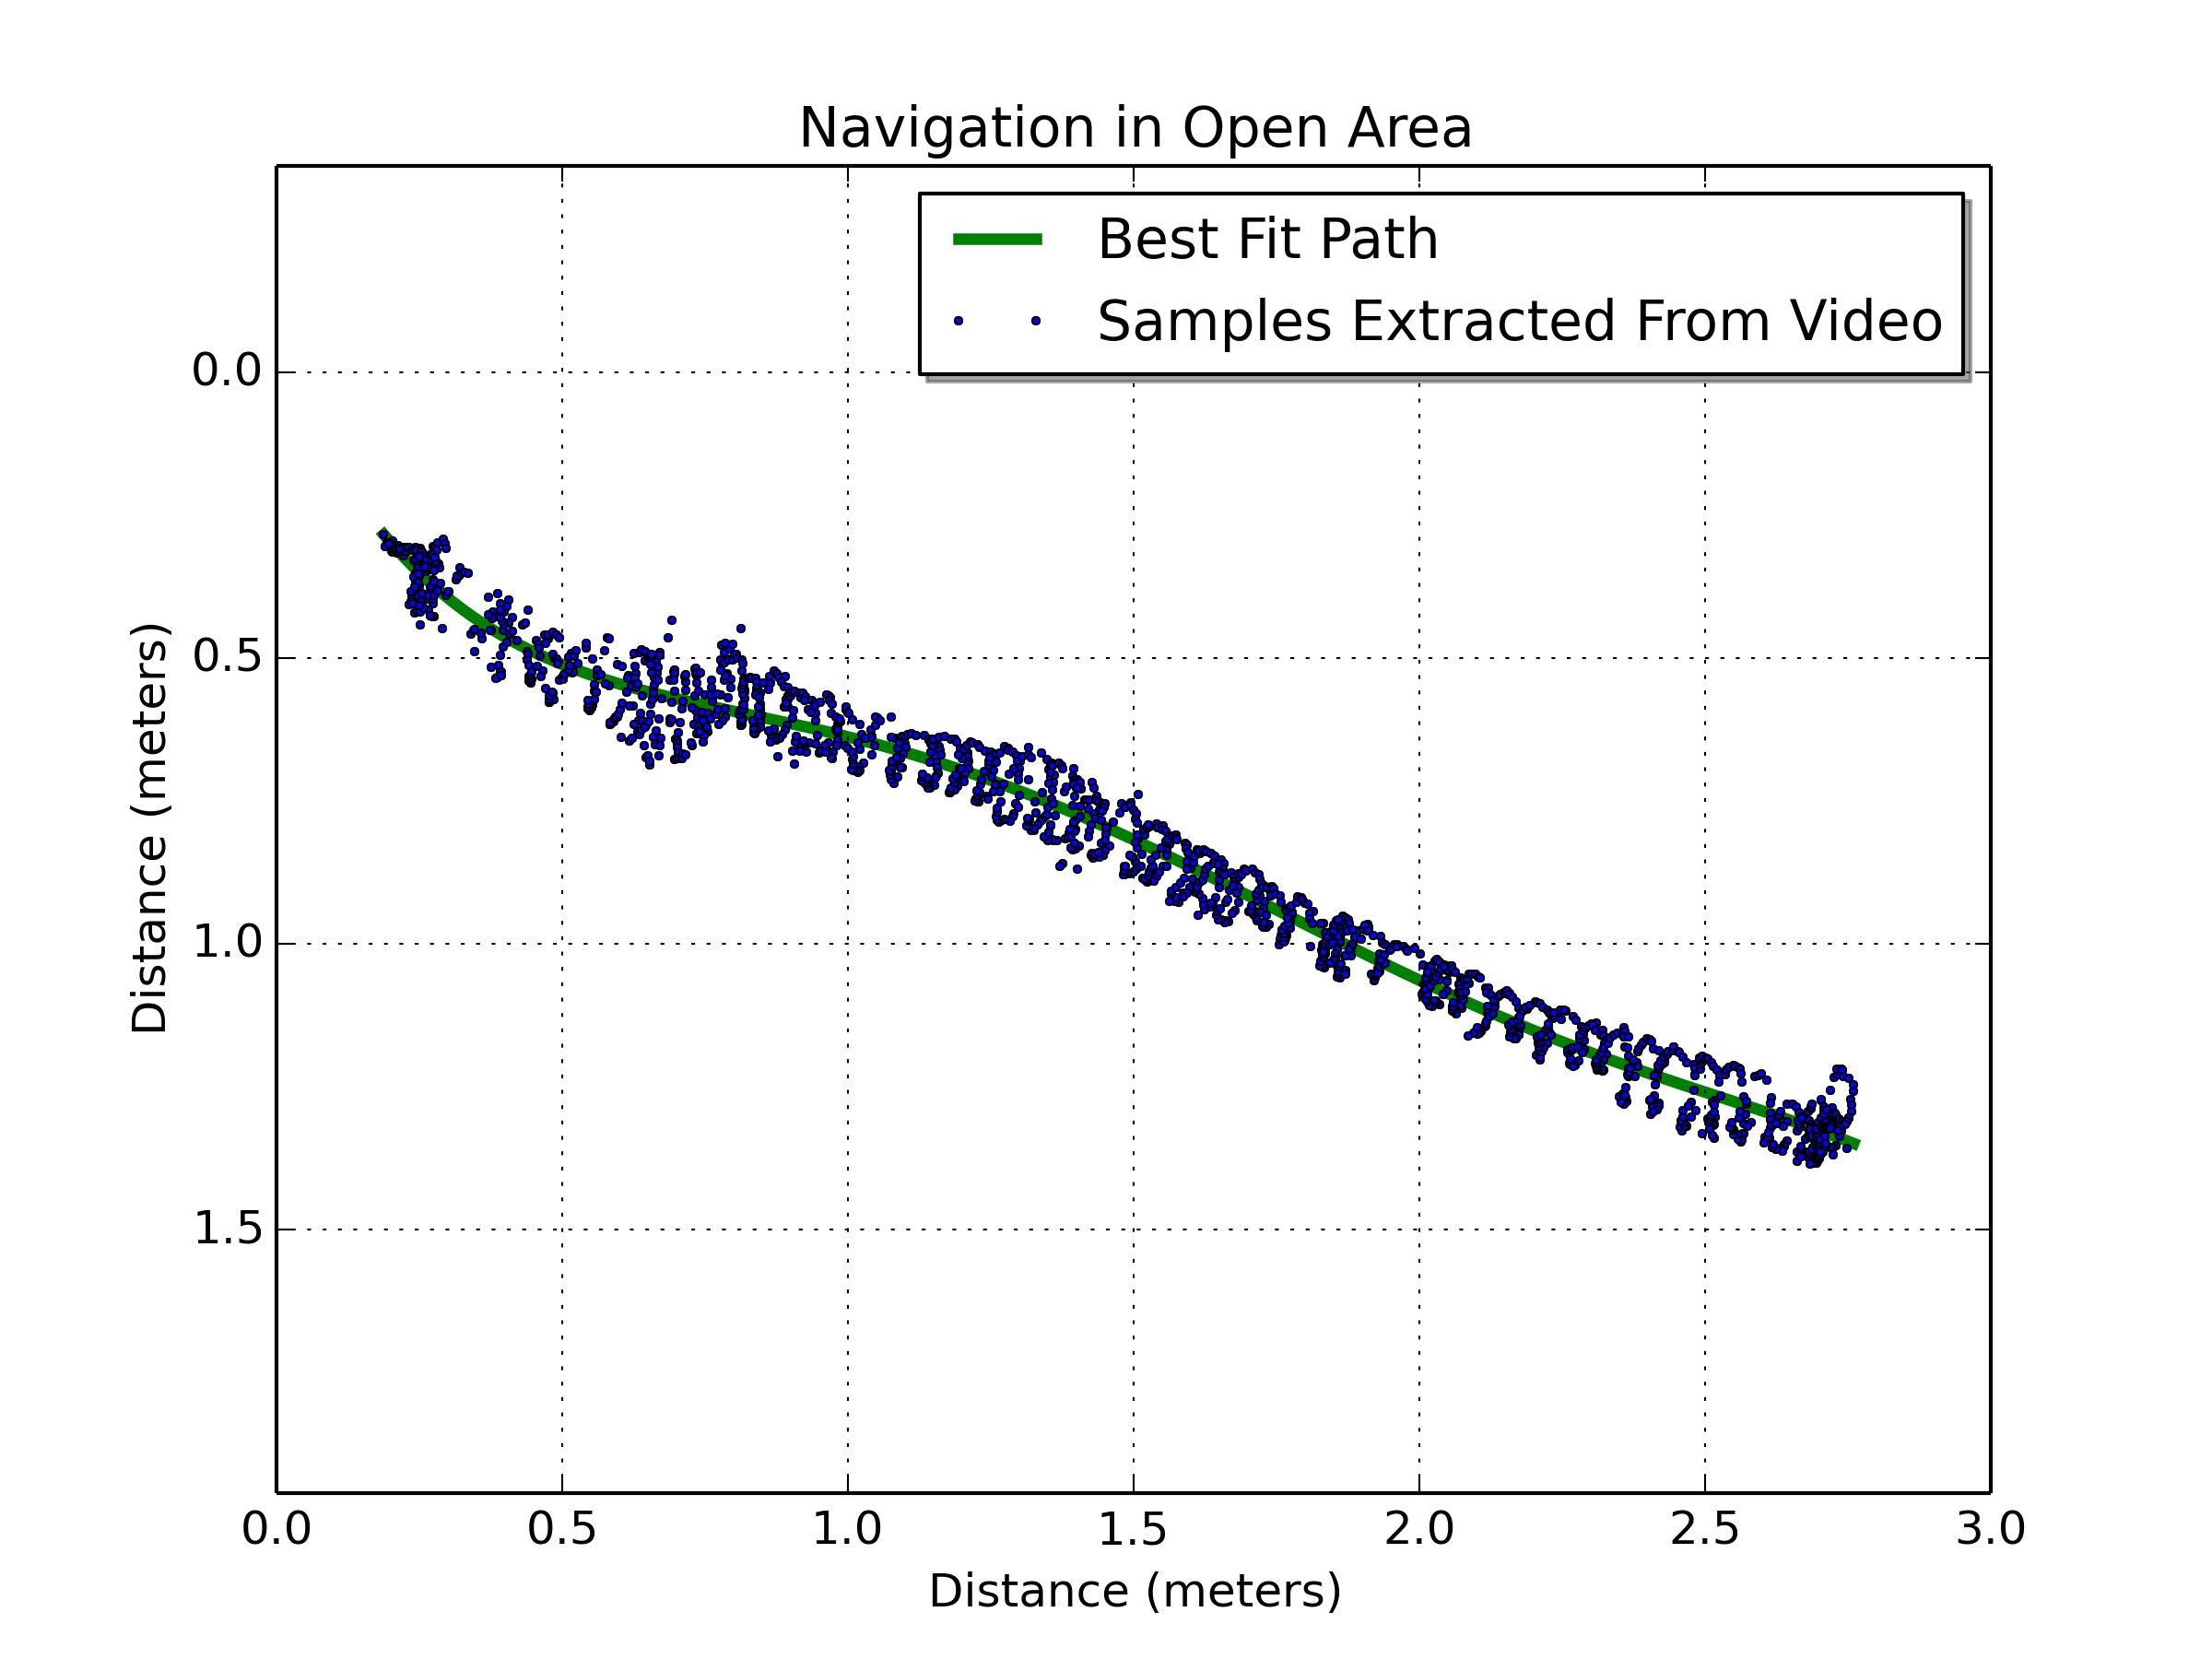
\includegraphics[height=0.35\textheight]{nav/open/plots/nav_open.png}
  \caption{This plot shows the centroid samples extracted from the global camera video from
           the open arena experiment. A fifth order polynomial has been fit to the samples
           and overlaid onto the plot.
           The robot starting point is shown as a red square on the left and the goal point 
           is shown as a yellow star on the right.
           The sample centroids clearly show the wobble in the gait.
           The robot stopped approximately $0.8 m$ from the goal.}
  \label{fig:nav_open_plot1}
\end{figure}

\begin{figure}
  \centering
  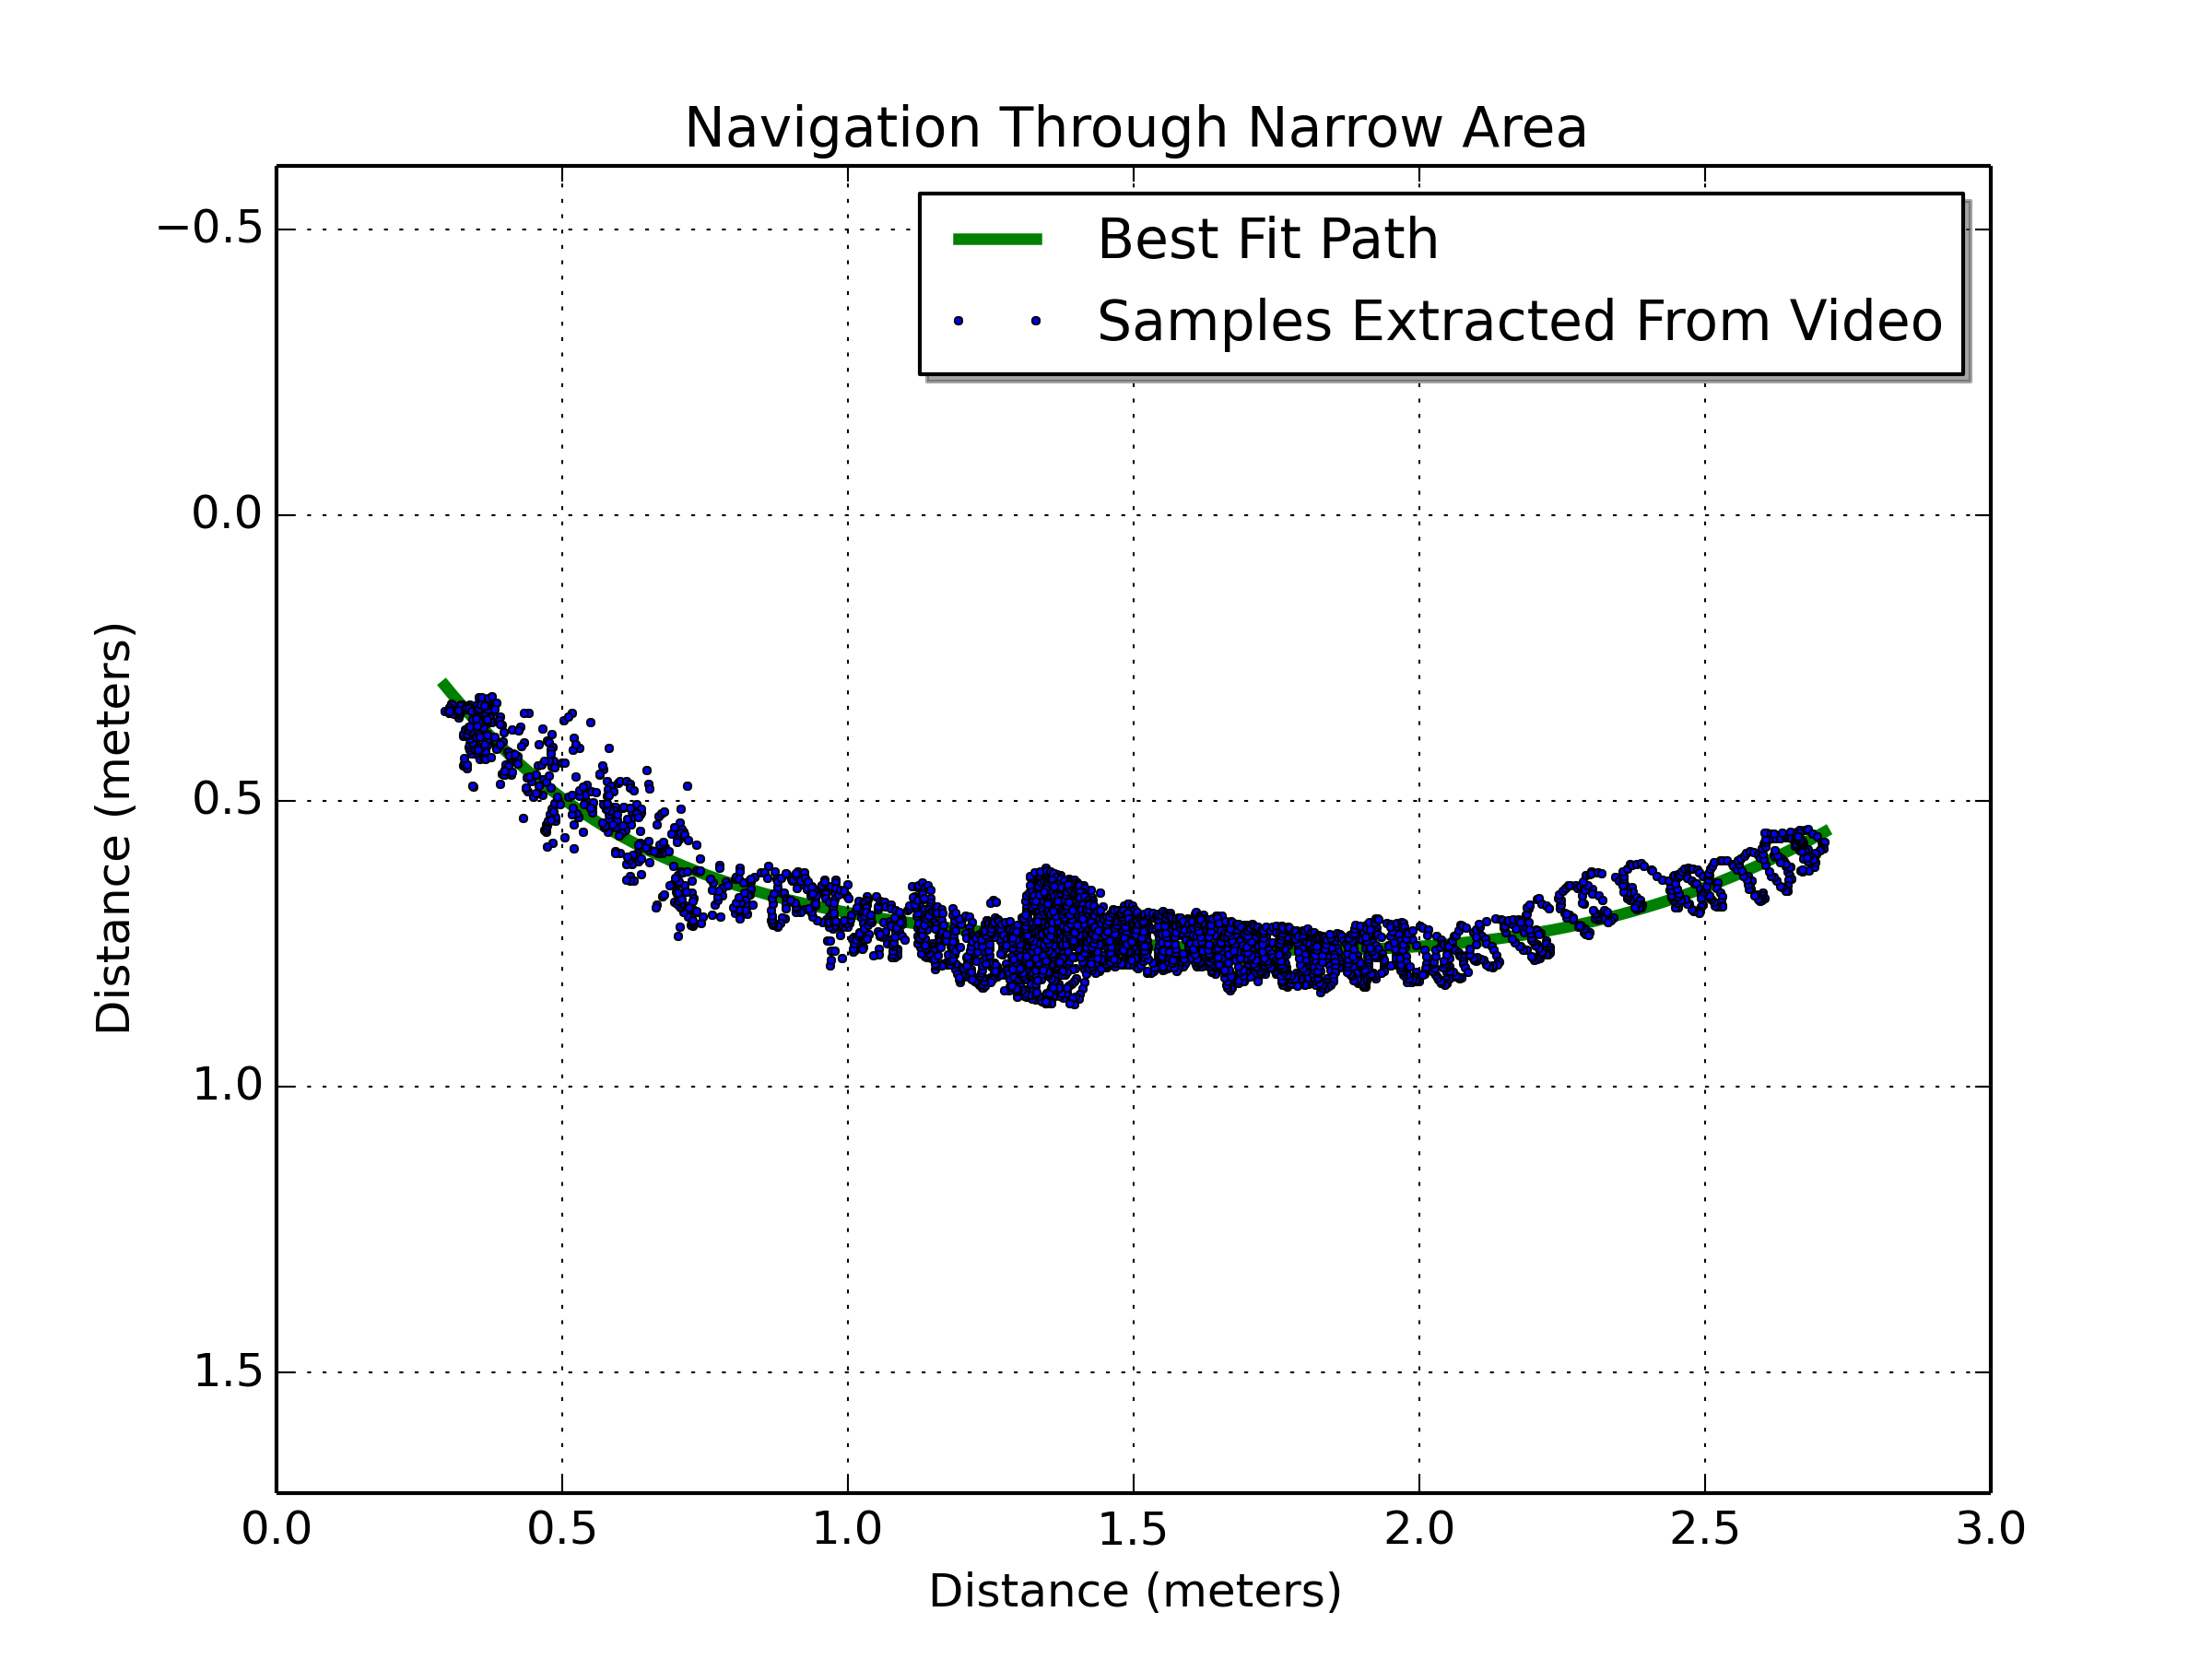
\includegraphics[height=0.35\textheight]{nav/narrow/plots/nav_narrow.png}
  \caption{This plot shows the centroid samples and best-fit path from the narrow opening arena experiment. 
           The oscillations shown by the samples can be seen to be the largest in the
           $(1.4, 0.75)$ region of the plot.}
  \label{fig:nav_narrow_plot1}
\end{figure}

\begin{figure}
  \centering
  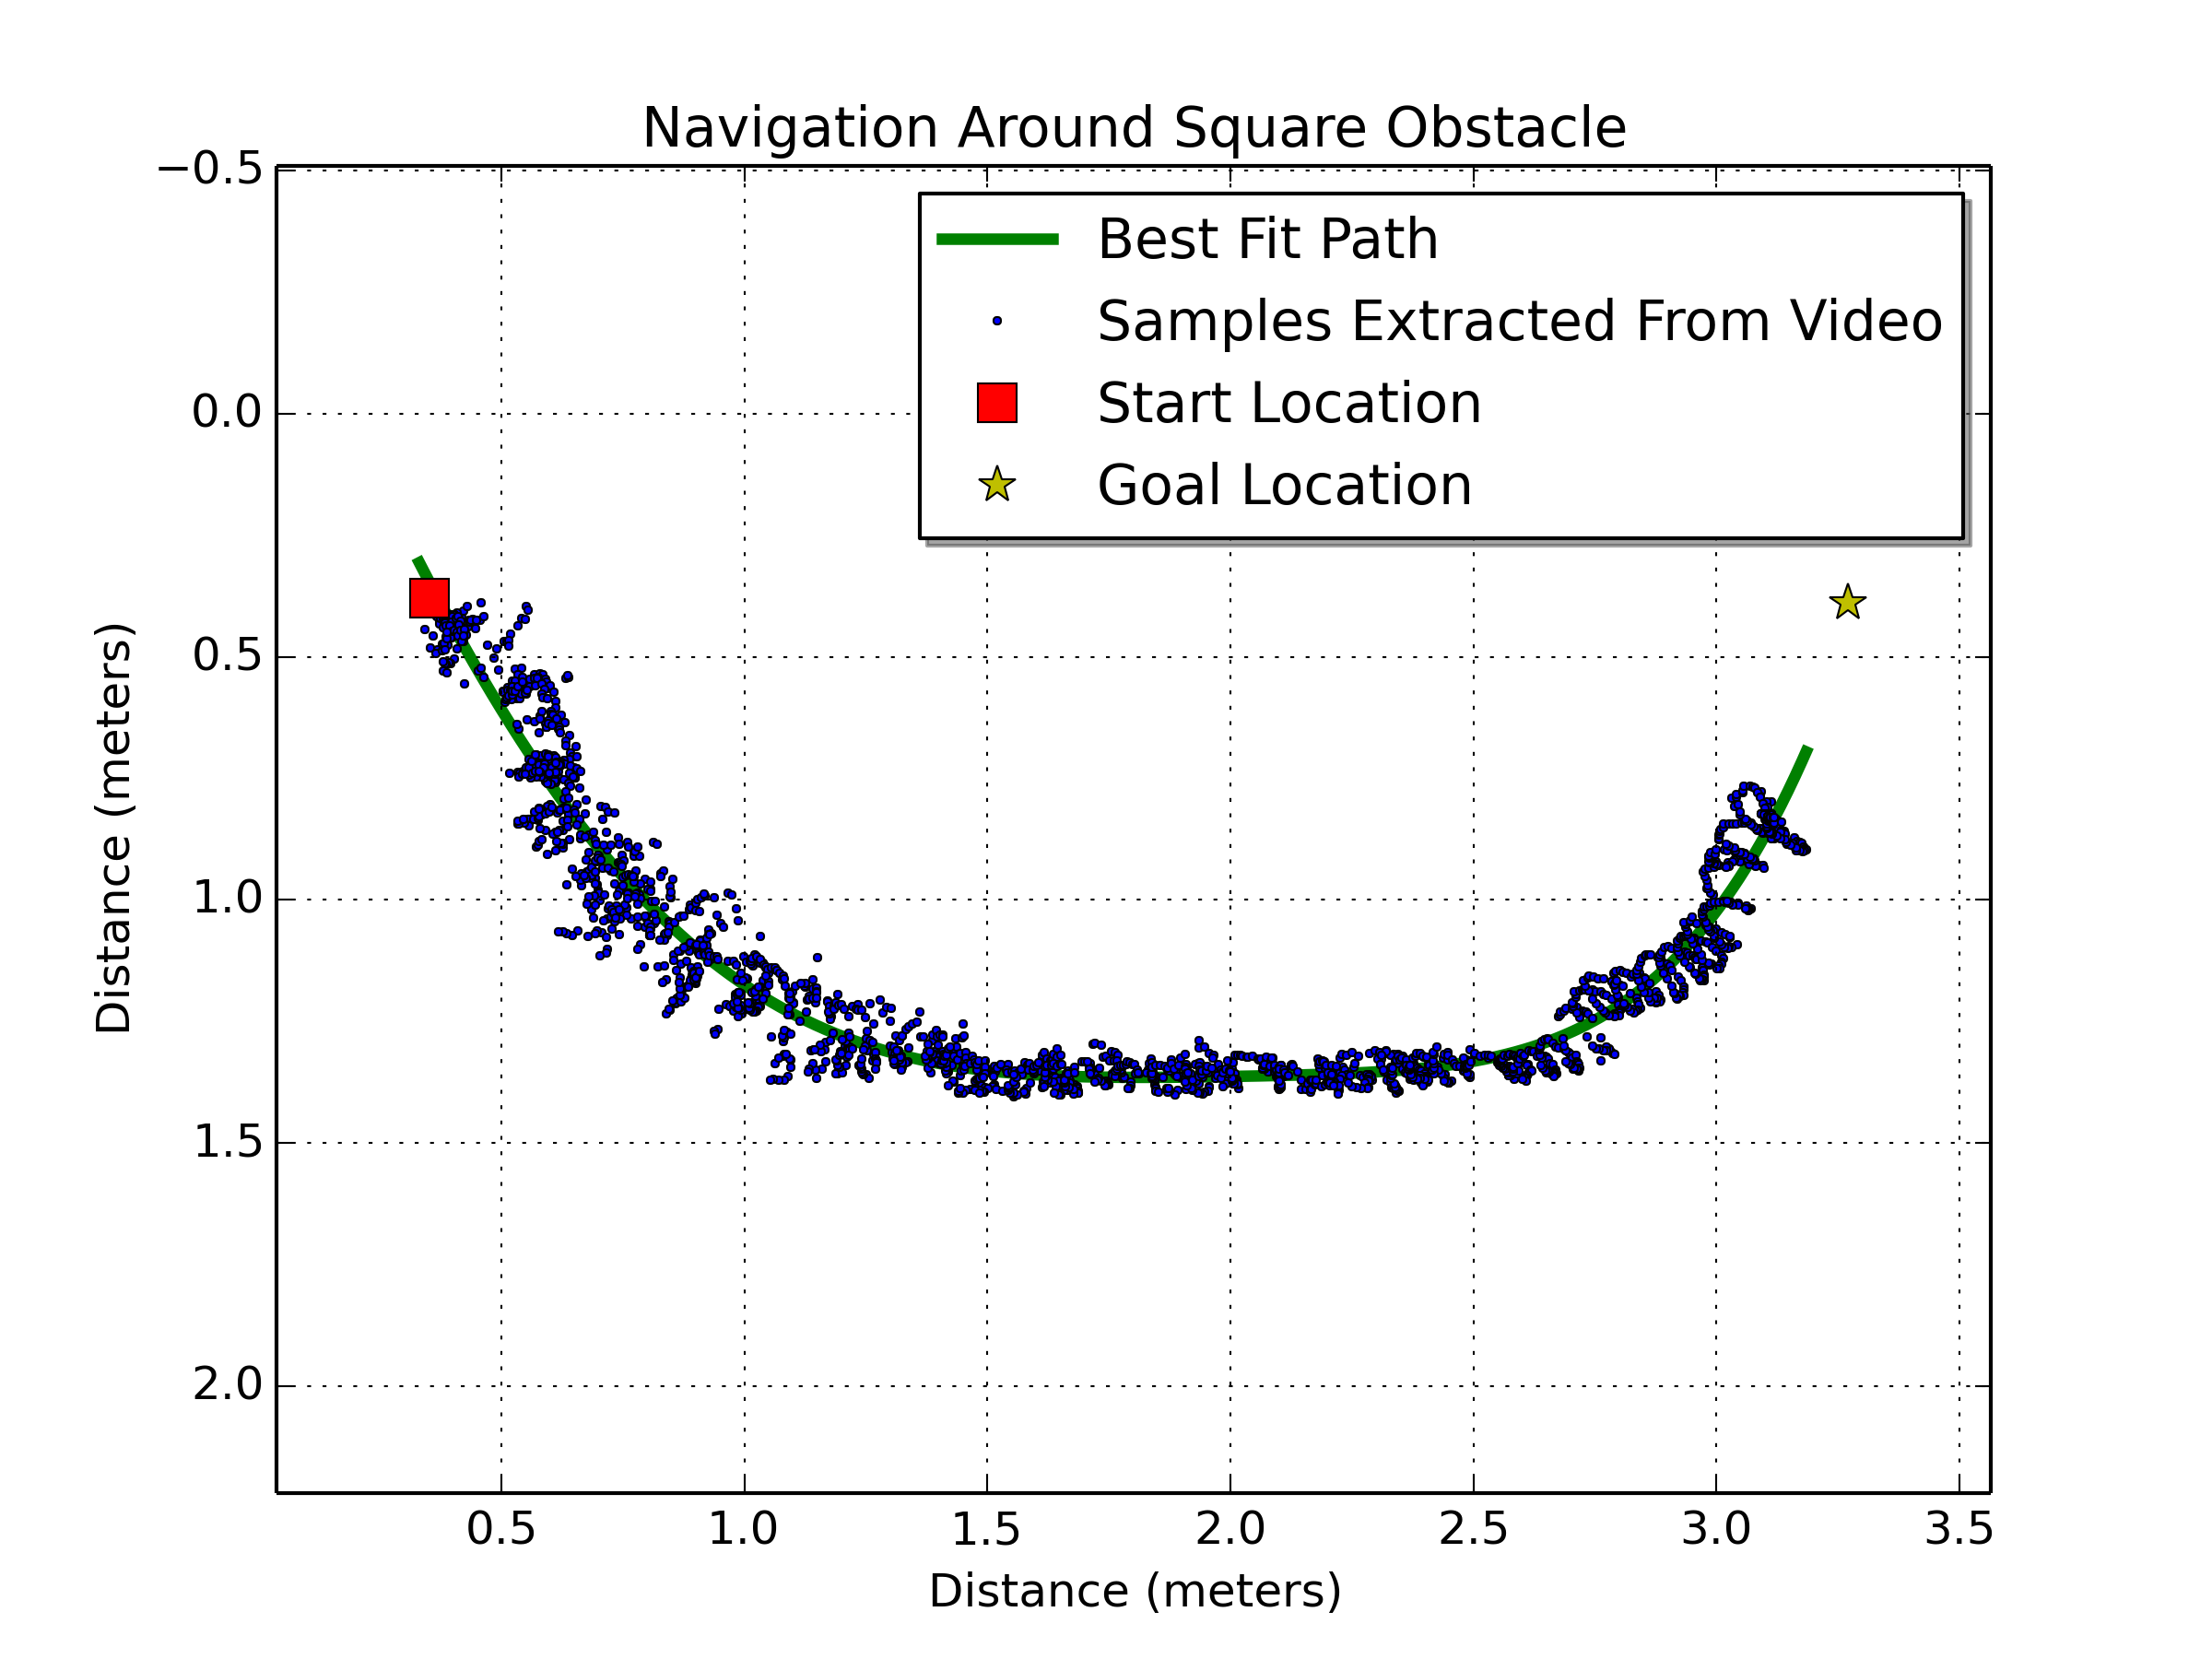
\includegraphics[height=0.35\textheight]{nav/square/plots/nav_square.png}
  \caption{This plot shows the centroid samples and best-fit path from the large obstacle arena experiment.
           The oscillations reduce along the path towards the bottom of the plot, but this is more of
           a limitation of the image processing procedure and when viewing the video, it is clear the oscillations
           are of similar magnitude to those seen in the rest of the experiment.}
  \label{fig:nav_square_plot1}
\end{figure}
